
\makeatletter
\def\@makechapterhead#1{%
  \centerline{{\fontsize{13pt}{13pt}\selectfont\underline{\LARGE\bf Deformations of Singularities}}}
  \vspace*{30\p@}%
  {\parindent \z@ \raggedright \normalfont
    \ifnum \c@secnumdepth >\m@ne
      \if@mainmatter
        \huge\bfseries Part\space \thechapter
       \par\nobreak
        \vskip 20\p@
      \fi
    \fi
    \interlinepenalty\@M
    \Huge \bfseries #1 \par\nobreak
    \vskip 40\p@
  }}
\makeatother

\chapter{Formal Theory and Computations}\label{part1}

\section{Definition of deformations}\label{part1-sec1}\pageoriginale

We work over an algebraically closed field $k$.

Let $X$ be an affine scheme, $X\hookrightarrow\mathbb{A}^{n}$. Let $A$
be finite (i.e., finite-dimensional/$k$) local algebra over $k$, so that
$A\approx k[t_{1},\ldots,t_{r}]/\mathfrak{a}$ with
$\sqrt{\mathfrak{a}}=(t_{1},\ldots,t_{r})$. Let $T=\Spec A$.

\begin{definition}\label{part1-defi1.1}%1.1
An {\em infinitesimal deformation} $X_{T}$(or $X_{A}$) of $X$ is a
scheme {\em flat}/$T$ together with a $k$-isomorphism
$X_{T}\times_{T}\Spec k \xrightarrow{\sim} X$.
\end{definition}

More generally, suppose we are given a commutative diagram
\[
\xymatrix{
X\ar[d]\ar@{^{(}->}[r]&\bar{X}\ar[d]^{\text{flat}}\\
\Spec k\ar[r]& \Spec R
}\]
where $R$ is a ring of finite type over $k$ and $\overline{X}$ is a scheme with closed fiber isomorphic to $X$. We then say that $\overline{X}$  is a {\em family of deformations} or a {\em deformation} of $X$ over $R$.

\begin{remark}\label{part1-rem1.1}%1.1
$X_{T}$ is necessarily affine. In fact $\exists$ a closed immersion $X_{T}\hookrightarrow\mathbb{A}^{n}_{T}(=\Spec A[X_{1},\ldots,X_{n}])$ such that its base change with respect to the morphism $\Spec k\rightarrow T$ (representing the closed point of $\Spec A$ is the immersion $X\hookrightarrow\mathbb{A}^{n}(=\mathbb{A}_{k}^{n})$.
\end{remark}

Let $\mathscr{O}=$ coordinate ring of $X$ and
$\mathscr{O}=k[X_{1},\ldots,X_{n}]/I$, with $x_{i}$ the
canonical\pageoriginale  images of $X_{i}$ in $\mathscr{O}$. To prove
the remark, it suffices to prove that if
$X_{A}\hookrightarrow\mathbb{A}_{A}^{n}$ is an affine scheme (over
$A$) imbedded in $\mathbb{A}_{A}^{n}, A'$ is a finite local
algebra/$k$ such that 
\begin{equation*}
0\rightarrow J \rightarrow A' \rightarrow A \rightarrow 0\quad \text{is exact}
\end{equation*}
with $J^{2}=0$ ($J$ is an ideal of square $0$) and $X_{A'}$ is a scheme/$A'$ such that $X_{A'}\times_{\Spec A'} \Spec A \simeq X_{A}$, then the immersion $X_{A}\hookrightarrow \mathbb{A}_{A}^{n}$ can be lifted to an immersion $X_{A'}\hookrightarrow\mathbb{A}_{A'}^{n}$. (This reduction is immediate since the maximal ideal is nilpotent. Say that $m_{A'}^{\rho}=0$, and take $J=m_{A'}^{\rho-1},\ldots)$. We have an exact sequence
\begin{equation*}
0\to I \to \mathscr{O}_{X_{A'}} \to \mathscr{O}_{X_{A}}\to 0,
\end{equation*}
where $\mathscr{O}_{X_{A'}}$, denotes the structure sheaf of $X_{A'}$. Now $I^{2}=0$ since $J^{2}=0$. This implies that $I$, which is {\em a priori} a (sheaf of) $\mathscr{O}_{X_{A'}}$ module(s), is in fact a module over $\mathscr{O}_{X_{A'}}/I$, i.e., it acquires a canonical structure  of coherent $\mathscr{O}_{X_{A}}$ -module. Since $X_{A}$ is affine, it follows that $H^{1}(X_{A'}, I)=0$ (for it is $=H^{1}(X_{A}, I)$). Hence
\begin{equation*}
  0\to H^{o}(X_{A'}, I)\to H^{o}(X_{A'}, X_{A'})\to H^{o}(X, X_{A})\to 0
\end{equation*}
is exact, i.e., in particular $H^{o}(X_{A'}, \mathscr{O}_{X_{A'}})\to H^{o}(X, \mathscr{O}_{X_{A}})\to 0$ is exact. Let $x_{i}$ be the coordinate functions on $X_{A}$ which define $X_{A}\hookrightarrow \mathbb{A}_{A}^{n}$. The $x_{i}$ can be lifted to $\xi_{i}\in H^{o}(X_{A'}, \mathscr{O}_{X_{A'}})$. Then the $\xi_{i}$ define a morphism $\xi:X_{A'}\to \mathbb{A}_{A'}^{n}$. It follows at first that $\xi$ is a {\em local} immersion; for this it suffices to prove that $\xi_{1}$\pageoriginale generate the local ring $\mathscr{O}_{X_{A',x}}$ at every closed point $x$ of $X_{A'}$. Let $I_{x}$ be the stalk of the ideal sheaf $I$ at a closed point $x$ of $X$. We have $0\to I_{x}\to \mathscr{O}_{A',x}\to\mathscr{O}_{A, x}\to 0(\mathscr{O}_{A', x'}\mathscr{O}_{A, x}$ represent the local rings at $x$ of $X_{A'}$ and $X_{A}$ respectively). We have $I_{x}=J\cdot\mathscr{O}_{A',x^{\cdot}}$. Now $j\cdot\theta_{1}=j\cdot\theta_{2}$ for $j \in J$ and $\theta_{1}, \theta_{2}$ in $\mathscr{O}_{A', x}$ such that their canonical images in $\mathscr{O}_{A, x}$ are the same. Let $S$ be the subalgebra of $\mathscr{O}_{A', x}$ generated by $\xi_{i}$ over $A'$. Then we see that $I_{x}=JS$. Since $J\subset A'$ it follows that $I_{x}\subset S$. Since $S$ maps onto $\mathscr{O}_{A, x'}$ given $\lambda\in\mathscr{O}_{A', x^{\cdot}}\exists s \in S$ such that $\lambda-s\in I_{x}$. This implies that $\lambda\in S$. This proves $S=\mathscr{O}_{A, x^{\cdot}}$. We conclude then that $\xi:X_{A'}\hookrightarrow \mathbb{A}_{A'}^{n}$ is a local immersion. But $\xi$ is a proper {\em injective} map (since $X_{A}\hookrightarrow_{A}^{n}$ is a closed immersion). From  this it follows that $\xi$ is a closed immersion. This proves the Remark.

Note that in the above proof we have {\em not used the fact} that $X_{A'}$ is {\em flat}/$A'$.

Given the closed subscheme $X\hookrightarrow \mathbb{A}_{k}^{n}$ let us define the following two functors on the category of finite local algebras over $k$.

\medskip
\noindent
$
\begin{matrix}
(\text{Def. } X) & : ~ (\text{Finite local alg}) \to (\text{Sets})\\
  | \; |
\end{matrix}
$

\noindent
\{Deformations of $X/A$\}$\mapsto$\{isom. classes (over $A$) of schemes $X$ flat/$A$ 

\hfill 
and  suct that $X_{A}\otimes k\simeq X$\}

\medskip

(Emb. def. $X$):(Finite local alg)$\to$(Sets)


\{Embedded deformations/$A\mapsto$ {closed subschemes $X_{A}$ of $\mathbb{A}_{A}^{n}$ flat/$A$, such that $X_{A}\hookrightarrow \mathbb{A}_{A}^{n}$ by base change is the given $X_{A}\hookrightarrow \mathbb{A}_{k}^{n}$\}

These\pageoriginale should be called respectively {\em infinitesimal deformations} of $X$ and {\em infinitesimal embedded deformations} of $X$. Then we have a canonical morphism of functors
$$
(Emb. def. X)\xrightarrow{f}(Def. X).
$$

The above Remark says that $f$ is {\em formally smooth}; that is, if
$A'\rightarrow A \rightarrow 0$ is exact in (Finite local alg), we
have 
$$
\xymatrix{
(Emb. def. X)(A')\ar[d] \ar[r] & (Def. X)(A')\ar[d]\\
(Emb. def. X)(A')\ar[r] & (Def. X)(A)
}
$$
(by definition of a morphism of functors), and the canonial map
$$
(Emb. def. X)(A')\rightarrow(Def. X)(A')\times_{(def. X)(A)}(Emb. def. X)(A)
$$
is {\em surjective}.

\section[Iarrobino's example of a 0-dimensional scheme...]{Iarrobino's example of a 0-dimensional scheme which is not a specialization of $d$ distinct points}\label{part1-sec2}

Given $X$ as above, we can ask whether it can be ``deformed'' into a nonsingular scheme. Here by a {\em deformation} we do not mean an infinitesimal one, but a general family of deformations. Let us consider the simplest case of Krull dimension $0$. Then $X=\Spec \mathscr{O}$ where $\mathscr{O}$ is a k-algebra of finite dimension $d$. If $d=1, \mathscr{O}\approx k$. If $d=2, \mathscr{O}\approx k \times k$ or $\mathscr{O}\approx k[t]/(t^{2})$. If $d=3$, we have
$$
\mathscr{O}=
\begin{cases}
k^{3}\quad \text{or}\quad k \times k[t]/t^{2}\\
\text{or}\quad k[t]/t^{3}\quad \text{or}\quad k[X, Y]/(X, Y)^{2}
\end{cases}
$$

In\pageoriginale our particular case the question is whether $X$ can be deformed into $d$ distinct points of $\mathbb{A}^{n}$. Now $\mathbb{A}^{n}\hookrightarrow \mathbb{P}^{n}$ and we see easily that this deformation implies a ``deformation'' of closed subschemes of $\mathbb{P}^{n}$, i.e., if $X$ can be deformed into $d$ ``distinct points'' we see (without much difficulty) that this can be done as an ``embedded deformation'' in $\mathbb{A}^{n}$ and in fact as an embedded deformation in $\mathbb{P}^{n}$. Let $\Hilb_{d}$ denote the Hilbert scheme of $0$-dimensional subschemes $Z\hookrightarrow\mathbb{P}^{n}$ such that if $Z=\Spec B$ then $B$ is of dim $d$ over $k$. Then it is known that $\Hilb_{d}$ is projective/$k$. Let $U_{d}$ denote the {\em open} sub-scheme of $\Hilb_{d}$ corresponding to $d$ distinct points, i.e., those closed sub-schemes of $\mathbb{P}^{n}$ corresponding to points of $\Hilb_{d}$ which are smooth. We see that $U_{d}$ is irreducible; in fact it is d-fold symmetric product of $\mathbb{P}^{n}$ minus the ``diagonals''. Now if every 0-dimensional subscheme can be deformed into a nonsingular one, then $U_{d}$ is dense in $\Hilb_{d}$ and it follow that $Hilb_{d}$ is {\em irreducible}.

We shall now give the counterexample (due to Iarrobino) where $\Hilb_{d}$ is {\em not} irreducible. It follows therefore that a 0-dimensional scheme cannot in general be deformed to a smooth one.

\begin{theorem}\label{part1-thm2.1}%2.1
Let $Hilb_{d,n}$ denote the Hilbert scheme of closed $0$-dimen\-sional subschemes of $\mathbb{P}^{n}$ of length $d$. Then $Hilb_{d,n}$ is {\em irreducible} for $n\le2$. For $n>2, \Hilb_{d,n}$ is {\em not} in general {\em irreducible}.
\end{theorem}

\begin{proof}
We give only the counter example for the case $n>2$. Let $\mathscr{O}^{'}=k[X_{1},\ldots,X_{n}]/(X_{1},\ldots,X_{n})^{r+1}$. Let $I$ be the ideal in $(X)^{r}/(X)^{r+1}$ (where $(X)=(X_{1},\ldots,X_{n})$). Then $I$ is a vector space over $k$ and
\begin{align*}
\text{Rank of}\quad I/k&=\text{Polynomial of degree}\quad (n-1)\quad \text{in}\quad r\\
\text{Rank of}\quad \mathscr{O}'/k&=\text{Polynomial of degree}\quad n\quad \text{in}\quad r.
\end{align*}\pageoriginale
\end{proof}

Now $I$ is an ideal in $\mathscr{O}'$ and in particular an $\mathscr{O}'$ module. Moreover, if $\lambda\in$ max ideal of $\mathscr{O}'$ then $\lambda \cdot I=0$. Hence $\mathscr{O}'$ operated on $I$ through its residue field. In particular, it follows that {\em any linear} subspace (over $k$) of $I$ is an ideal in $\mathscr{O}'$ and hence defines a closed subscheme of $\Spec \mathscr{O}'$. Take now $\theta=\frac{1}{2}$ Rank $I$ or $\frac{1}{2}$ Rank $I-\frac{1}{2}$ according as Rank $I$ is even or odd and $d=\text{Rank}(\mathscr{O}'/V)$, where $V$ is a subspace of $I$ of rank $\theta$. Hence $\theta=\text{Polynomial of degree}(n-1)$ in $r$ and $d=\text{polynomial of degree } n \text{ in } r$. Let us now count the dimension of the set $L_{\theta}$ of all linear subspaces of $I$ of rank $=\theta$. Then it is a Grassmannian and $dim L_{\theta}=\left(\frac{1}{2}\text{ Rank } I\right)^{2}$ or $\left(\frac{1}{2} \text{ Rank } I-\frac{1}{2}\right)\left(\frac{1}{2}\text{ Rank } I+\frac{1}{2}\right)$ according as Rank $I$ is even or odd$=$(Polynomial of $deg \;  n-1)^{2}$ in $r=$ {\em Polynomial of degree} ($2n-2$) {\em in} $r$. Now if $U_{d}$ is the subscheme of $\Hilb_{d}$ of ``d distinct points'' as above, then
$$
\dim U_{d}=d.n=n(\text{Polynomial of degree}\quad n\quad \text{in}\quad r).
$$

Now if $r\gg0$, we see that
$$
\dim L_{\theta}> \dim U_{d}.
$$

Since $L_{\theta}$ can be identified as a subscheme of $\Hilb_{d}$, it
follows now that $U_{d}$ is {\em not} dense in $\Hilb_{d}$. To see
that $L_{\theta}$ is a subscheme of $Hilb_{d}$, note that $\Spec
\mathscr{O}/I$ as a point set consists only of one point. The family
of subschemes of $\mathbb{P}^{n}$ parametrized by $L_{\theta}$ as a
point given by $(x_{o}\times L_{\theta})$. It suffices to check that
on $(x\times L_{\theta})$, we have a natural structure of a scheme
$\Gamma$ such that  
\begin{center}
\centering
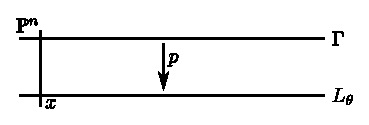
\includegraphics{figure/chap1-fig1.eps}
\end{center}
$\Gamma$ is a closed subscheme of $\mathbb{P}^{n}\times L_{\theta}$ and $p^{-1}(x)$ is the subscheme of $\Spec \mathscr{O}/I$ defined by the linear subspace\pageoriginale of $I$ corresponding to $x$. Then we see that $p:\Gamma \rightarrow L_{\theta}$ is flat, for $p$ is a finite morphism over $L_{\theta}$ such that $\mathscr{O}_{\Gamma}$ is a sheaf of $\mathscr{O}_{L_{\theta}}$ -algebras; in particular, $\mathscr{O}_{\Gamma}$ becomes a coherent sheaf over $\mathscr{O}_{L_{\theta}}$. At every $x\in L_{\theta}$, for $\mathscr{O}_{\Gamma}\otimes\mathscr{O}_{L_{\theta}}, x/\text{maxideal} (=\mathscr{O}_{\Gamma}\otimes k)$, the rank is the same. $L_{\theta}$ is reduced, this implies that $\mathscr{O}_{\Gamma}$ is locally free over $\mathscr{O}_{L_{\theta}}$. In particular, $\Gamma$ is flat/$L_{\theta}$.

\section{Meaning of flatness in terms of relations}\label{part1-sec3}

A module $M$ over a ring $A$ is said to be {\em flat} if the functor $N\mapsto M\otimes_{A}$ is {\em exact}.
\begin{align*}
\Leftrightarrow Tor_{q}^{A}(M, N)&=0\quad\forall N/A.\\
\Leftrightarrow Tor_{l}^{A}(M, N)&=0\quad \forall \text{finitely generated} N/A.
\end{align*}

Let us now consider the case when $A$ is  a finite {\em local} $k$-{\em algebra}. Then if $N$ is an $A$-module of finite type, there is a composition series
$$
N=N_{0}\supset N_{1}\supset\ldots\supset N_{\ell}=0,\quad \text{such that}\quad N_{i}/N_{i}+1\approx k.
$$

From this it follows immediately that

$$
M flat/A \Leftrightarrow Tor_{1}(M, k)=0\quad(\text{if $A$ finite local } alg/k).
$$

Let $X_{A}=\Spec \mathscr{O}_{A}$, A {\em finite local algebra} and $\mathscr{O}_{A}$ an A-algebra of {\em Iinite type} so that we have

$$
0\rightarrow I_{A}\rightarrow P_{A}\rightarrow \mathscr{O}_{A}\rightarrow 0
$$
exact with $P_{A}A[X] (X=(X_{1},\ldots,X_{n}))$. Tensor this with $k$. Then we have
$$
o\rightarrow Tor_1(\mathscr{O}_A, k)\rightarrow I_A \otimes k\rightarrow P_k\rightarrow \mathscr{O}_k\rightarrow 0 
$$\pageoriginale

Let $X=\Spec \mathscr{O}_k$, $X\approx X_A \otimes k$, $I$ ideal of $X$ in $\mathbb{A}^n$. Then
\begin{align*}
X_A \text{is flat}/A &\Leftrightarrow Tor_1(\mathscr{O}_A, k)=0,\\
&\Leftrightarrow I_A \otimes k=I.
\end{align*}

Take a presentation for the ideal $I_A$ in $P_A$, i.e., an exact sequence
\begin{equation*}
\vcenter{
\xymatrix{
P_A^\ell\ar[r] & P^{m}_{A}\ar[rr]\ar[dr] & & P_{A}\ar[r] & \mathscr{O}_{A}\ar[r] & 0\\
 & & I_{A}\ar[ur]\ar[dr] & & &\\
 & 0\ar[ur] & & 0 & &
}}\tag{*}
\end{equation*}

{\em Then we have (because of the above facts)}: $\mathscr{O}_A$ is $A$-{\em flat} $\Leftrightarrow$ {\em the above presentation for} $I_{A}$ tensored by $k$, {\em gives a presentation for} $I$, i.e., {\em tensored by} $k$ {\em gives again an exact sequence}
\begin{equation*}
\vcenter{
\xymatrix{
P_k^\ell\ar[r] & P^{m}_{k}\ar[rr]\ar[dr] & & P_k \ar[r] & \mathscr{O}\ar[r] &0\\
& & I \ar[ur]\ar[dr] & & &\\
& 0\ar[ur] & & 0  &  &}}\tag{**}
\end{equation*}

{\em Suppose we are given:}

$\mathscr{O}=K[X]/(f_1,\ldots,f_m)$ and liftings $(f'_i)$ of $(f_i)$ to elements in $A[X]$. Let $I=(f_1,\ldots,f_m)$, $I_A=(f'_1,\ldots,f'_m)$ and $\mathscr{O}_A=A[X] (f'_1,\dots,f'_m)$. These data are equivalent to giving a lifting $P_A^m\rightarrow P_A\rightarrow \mathscr{O}_A\rightarrow 0$ of the exact sequence $P^m\rightarrow P\rightarrow \mathscr{O}\rightarrow 0$, i.e., to giving an {\em exact sequence} $P_A^m\rightarrow P_A \rightarrow \mathscr{O}_A\rightarrow 0$ such that\pageoriginale its $\otimes_A k$  is the given exact sequence $P^{m}\rightarrow P\rightarrow\mathscr{O}\rightarrow 0$. {\em Note that this need not imply that} $I_A \otimes k=I$ {\em if} $I_A=\Ker(P_A\rightarrow \mathscr{O}_A)$ {\em and} $I=\Ker(P\rightarrow \mathscr{O})$.

Suppose we are now given a ``complete set of relations'' (or a presentation for $I$) between $f_i$'s, i.e., an {\em exact  sequence}
\begin{equation*}
P^{\ell}\rightarrow P^{m}\rightarrow P \rightarrow \mathscr{O}\rightarrow 0.\tag{*}
\end{equation*}

Then {\em giving a lifting of these relations} to that of $f_{i}^{'}$'s (or $I_A$) is to give
\begin{equation*}
P_A^{\ell}\rightarrow P_A^{m}\rightarrow P_A \rightarrow \mathscr{O}_A\rightarrow 0\tag{**}
\end{equation*}
which extends the exact sequence $P_A^{m}\rightarrow P_A\rightarrow \mathscr{O}_A\rightarrow 0$, which is a {\em complex} at $P_A^{m}$, i.e., $Im P_A^{\ell}\subset \Ker(P_A^{m}\rightarrow P_A)$ and such that $(**)$ lifts $(*)$. In this situation we have the following 

\begin{proposition}\label{part1-prop3.1}%3.1
Suppose
\begin{equation*}
P^{\ell}\rightarrow P^{m}\rightarrow P \rightarrow \mathscr{O}\rightarrow 0\tag{*}
\end{equation*}
is {\em exact} and
\begin{equation*}
P_A^{\ell}\rightarrow P_A^{m}\rightarrow P_A \rightarrow \mathscr{O}_A\rightarrow 0\tag{**}
\end{equation*}
is a {\em complex} such that the part
$$
P_A^{m}\rightarrow P_A \rightarrow \mathscr{O}_A\rightarrow 0
$$
is exact and (**) $\otimes_A k=(*)$. Then $\mathscr{O}_A$ is $A$-flat.
\end{proposition}

\begin{proof}
Suppose first that
\begin{equation*}
P_A^{\ell}\rightarrow P_A^{m}\rightarrow P_A \rightarrow \mathscr{O}_A\rightarrow 0\tag{*}
\end{equation*}\pageoriginale
is exact not merely a ``complex at $P_A^{m_{11}}$. Then we claim that the flatness of $\mathscr{O}_A$ over $A$ follows easily. For then (**) can be split up as:
\begin{equation*}
\left.
\begin{aligned}
P_A^{\ell}\rightarrow &L_A\rightarrow 0,\quad 0\rightarrow L_A \rightarrow P_A^{m}\rightarrow I_A \rightarrow 0\\
&0\rightarrow I_A\rightarrow P_A \rightarrow \mathscr{O}_A \rightarrow 0
\end{aligned}
\right\}
\quad\text{exact.}
\end{equation*}

Therefore $P_A^{\ell}\otimes k\rightarrow L_A \otimes k\rightarrow 0$
and $L_A\otimes k\rightarrow P_A^{m}\otimes k\rightarrow 0$ are
exact. This implies that $I_A\otimes k=\text{coker}(k\otimes
P_A^{\ell}\rightarrow k\otimes P_A^{m}$)m i.e., cokernel is pre-served
by $k\otimes_A$. On the other hand,
$I=\text{Coker}(P^{\ell}\rightarrow P^{m})$. Hence $I_A\otimes
k=I$. {\em From this it follow that} $\mathscr{O}_A$ {\em is flat/A as
remarked before}. Now the hypotheses of our proposition amount to the
fact all relations in $I$ can be lifted to $I_A$. Given a relation in
$I_A$, i.e., an $m$-tuple $(\lambda'_1,\ldots,\lambda'_m)$ such
that $\sum\lambda'_{i}f'_{i}=0$, this descends to a relation in
$1$ by taking the canonical images of $\lambda^{'}_i$ in $P$. Take a
complete set of relations for $I_A$, i.e., an exact sequence 
\begin{equation*}
P_A^{\ell'}\rightarrow P_A^{m}\rightarrow P_A\rightarrow \mathscr{O}_A\rightarrow 0\qquad (\ell^{'}\quad \text{need not be}\quad\ell),\tag{i}
\end{equation*}
then from our above argument this descends to a complete set of relations for $I$, i.e., tensoring (i) by $k$ we get an exact sequence
\begin{equation*}
P^{\ell^{'}}\rightarrow P^{m}\rightarrow P \rightarrow \mathscr{O}\rightarrow 0.
\end{equation*}

Consequently, we have already shown in this situation that we must have $\mathscr{O}_A$ to be A-flat.
\end{proof}

The criterion for flatness can given be formulated as follows:

\begin{coro*}
Let\pageoriginale $\mathscr{O}=k[X]/(f_1,\ldots,f_m)$ and $\mathscr{O}_A=A[X]/(f^{'}_1,\ldots,f^{'}_m)$ where $f^{'}_i$ are liftings of $f_i$. Then
$\mathscr{O}_A$ is A-flat $\Leftrightarrow$ every relation among $(f_1,\ldots,f_m)$ lifts to a relation among $(f^{'}_1,\ldots,f^{'}_m)$.
\end{coro*}

\begin{remark}\label{part1-rem3.1}%3.1
It is seen immediately that
$$
\mathscr{O}_A\text{flat}/A\Rightarrow I_A \text{flat}/A.
$$

For, the exact sequence $0\rightarrow I_A \rightarrow
P_A \rightarrow \mathscr{O}_A\rightarrow 0$ by tensoring by $k$ gives 
{\fontsize{10}{12}\selectfont
\begin{equation*}
\xymatrix@R=0.8pc@C=0.7pc{
0\ar @{} [d]|{\parallel} & & 0 \ar @{} [d]|{\parallel} & 0 \ar @{} [d]|{\parallel}\\
\text{Tor}_2(\mathscr{O}_A, k)\ar[r]& \text{Tor}_1(I_A, k)\ar[r]
& \text{Tor}_1(P_A, k)\ar[r]& \text{Tor}_1(\mathscr{O}_A, k)\ar[r]
&1 \ar[r]& P_k\ar[r]&\mathscr{O}\ar[r]& 0} 
\end{equation*}}\relax
This implies that $\text{Tor}_1(I_A, k)=0$, hence that $I_A$ is
flat/$A$, by a previous Remark. Repeating the procedure for
$\mathscr{O}_A$, we see by succesive reasoning that any {\em
resolution} for $\mathscr{O}$ lifts to one for $\mathscr{O}_A$. 
\end{remark}


\section{Deformations of complete intersections}\label{part1-sec4}

Let $X\hookrightarrow \mathbb{A}^{n}$ be a complete intersection. Let $d=\text{dim} X$ (Krull dim) and $I=(f_1,\ldots,f_{n-d})$ the ideal of $X$. Let $\mathscr{O}=P/I$, where $P=P_k=k[X_1,\ldots,X_n]$ Then it is well known that the ``Koszul complex'' gives a resolution for $\mathscr{O}$, i.e.,
$$
\displaystyle\mathop\wedge^{2}P^{n-d}\rightarrow \displaystyle\mathop\wedge^{1}P^{n-d}(=P^{n-d})\rightarrow
P \rightarrow \mathscr{O}\rightarrow 0 
$$
the homomorphisms being interior multiplication by the vector\pageoriginale 
$$
(f_1,\ldots,f_{n-d})\in P^{n-d},
$$ 
(e.g., $P^{n-d}\rightarrow P$ is the map
$(\lambda_1,\ldots,\lambda_{n-d})\mapsto\sum_i\lambda_if_i$). The
image of $\displaystyle\mathop\wedge^{2}P^{n-d}$ in $P^{n-d}$ gives
the realtions in $I$, which shows that the relations among the $f_i$
are (generated by) the obvious ones, i.e., $f_i z_j-f_jz_i=0$. 

Let $A=k[t]/(t^{2})$ ({\em which we write} $A=k+kt$ {\em with}
$t^{2}=0)$. {\em Then deformations of $X$ over $A$ are called first
order deformations}. Lert $I_A$ be the ideal in $A[X_1,\ldots,X_n]$. 
$$
I_A=((f_1+g_1t),\ldots,(f_{n-d}+g_{n-d}t))
$$
where $g_i\in P_k$. We {\em claim} that {\em for arbitrary choice of}
$g_i \in P_k, \mathscr{O}_A=P_A/I_A$ is {\em flat} over $A$ (of course
we have seen that any deformation $X_A$ of $X$ can be defined by $I_A$
for sutiable choice of $g_i$). This is an immediate consequence of the
fact that above {\em explicit relations} between $f_i$ can obviously
be lifted to relations between $(f_i+g_it)$. This proves the claim. 

Thus to classify embedded first order deformations it suffices to
write down conditions on $(g_i), (g^{'}_i)$ in $P$ so that in $P_A$
the ideals $((f_i+g_it))$ and $((f_i+g^{'}_it))$ are the same. {\em We
claim}: 
$$
((f_i+g_it))=((f_i+g_i^{'}t))\Leftrightarrow g_i-g_i^{'}\in I.
$$

To prove this we proceed as follows:
\begin{align*}
((f_i+g^{'}_i&t))\subset((f_i+g_it))\Leftrightarrow\qquad(\text{Set}\quad r=n-d.)\\
f_i+g^{'}_it&=\sum\limits_{j=1}^{n-d}(\alpha_{ij}+\beta_{ij}t)(f_j+g_jt)\\
   &=\left(\sum\limits_{j=1}^{r}\alpha_{ij}f_{j}\right)+t\left(\sum\limits_{j=1}^{r}\alpha_{ij}g_j+\sum\limits_{j=1}^{r}\beta_{ij}f_{j}\right)\Leftrightarrow
\end{align*} 

$\exists$\pageoriginale ($r\times r$) matrices $(\alpha_{ij})$ and $(\beta_{ij})$ with coefficients in $P$ such that
\begin{enumerate}[(a)]
\item $(\alpha_{ij}) \begin{bmatrix}
f_{1}\\
\vdots\\
f_{r}
\end{bmatrix}=\begin{bmatrix}
f_1\\
\vdots\\
f_r
\end{bmatrix}, \text{i.e.,}(\alpha_{ij}-Id)\displaystyle\mathop{(\vdots)}^{f_1}_{f_r}=(0),\text{and}
$
\item $(\alpha_{ij})\begin{bmatrix}
g_1\\
\vdots\\
g_r
\end{bmatrix}+(\beta_{ij})\begin{bmatrix}
f_1\\
\vdots\\
f_r
\end{bmatrix}=\begin{bmatrix}
g_{1}^{'}\\
\vdots\\
g_{r}^{'}
\end{bmatrix}$.
\end{enumerate}

Since the coordinates of the relation vectors are in $I$ it follows from $(a)$ above that the element of $(\alpha_{ij}-Id)$ are in $I$, i.e., $(a)\Rightarrow (\alpha_{ij})\equiv(Id)\mod I)$. Then $(b)$ implies that
$$
\begin{bmatrix}
g_1\\
\vdots\\
g_r
\end{bmatrix}\equiv\begin{bmatrix}
g_{1}^{'}\\
\vdots\\
g_{r}^{'}
\end{bmatrix} 
(\text{mod\,} I).
$$

Hence $((f_i+g_{i}^{'}))\subset((f_i+g_it)\Rightarrow(g_i-g_{i}^{'})\in I$. Hence $((f_i+g_it))=((f_i+g_{i}^{'}t))\Rightarrow (g_i-g_{i}^{'})\in I$. Conversely, suppose that $(g_i-g_{i}^{'})\in I$. Then there is a matrix $(\beta_{ij})$ such that
\begin{equation*}
(\beta_{ij}\begin{bmatrix}
f_1\\
\vdots\\
f_r
\end{bmatrix}=\begin{bmatrix}
g_{1}^{'}\\
\vdots\\
g_{r}^{'}
  \end{bmatrix}-\begin{bmatrix}
g_1\\
\vdots\\
g_r
  \end{bmatrix}
\end{equation*}

Hence, $(Id)\begin{bmatrix}
g_1\\
\vdots\\
g_r
\end{bmatrix}+(\beta_{ij})\begin{bmatrix}
f_1\\
\vdots\\
f_r
\end{bmatrix}=\begin{bmatrix}
g_{1}^{'}\\
\vdots\\
g_{r}^{'}.
\end{bmatrix}
$ 

Taking $(\alpha_{ij})=Id$ we see that the conditions $(a), (b)$ are
satisfied, which implies that $((f_i+g_it))=((f_i+g^{'}_{i}t))$. This
proves the claim and thus we have classified {\em all
embedded}\pageoriginale ({\em in} $\mathbb{A}^{n}$) {\em first order
deformations of} $X$. 

Now to classify first order deformations of $X$ we have only to write
down the condition when two embedded deformations $X_A, X'_{A}$ are
isomorphic over $A$. Let $\theta$ be an isomorphism
$X_A \xrightarrow{\sim} X_{A}^{'}$. By assumption, $X\otimes k=
X_{A}^{'}\otimes k=X$. i.e., their fibres over the closed point of
$\Spec A$ are $X\subset \mathbb{A}^{n}$. We denote (of course) by
$X_\nu$ the canonical coordinate functions of
$X_A\hookrightarrow \mathbb{A}_{A}^{n}=\Spec A[X_1,\ldots, X_n]$. Let
$X_{\nu}^{'}=\theta^{\star}(X_\nu)$. Then we have 
$$
X_{\nu}^{'}=X_{\nu}+\varphi_{\nu}(X)t
$$
for some polynomials $\varphi_{\nu}(X)$. Hence to identify two
embedded deformations of $X$ we have to consider the identification by
the above change of coordinates. Then 
$$
f_i+g_it\mapsto f_i(X_{\nu}+\varphi_{\nu}(t))+g_i((X_{\nu}+\varphi_{\nu}(t))t.
$$

By Taylor expansion up to the first order, we get
\begin{align*}
&=f_i(X)+t\left\{\displaystyle\mathop{\sum}_{\nu}\frac{\partial
f_i}{\partial X}\varphi_{\nu}(X)\right\}+tg_i(X)\\ 
&=f_i(X)+t\left\{g_i(X)+\sum_{\nu=1}^{n}\frac{\partial f_i}{\partial X}\varphi_{\nu}(X)\right\}
\end{align*}

Hence $(f_i+g_it)$ and $(f_i+g_{i}^{'}t)$ define the same deformation
of the first order up to change of coordinates above, which is
equivalent to the fact that there exists
$(\varphi_1,\ldots,\varphi_n)$ such that 
\begin{equation*}
\begin{bmatrix}
g_1\\
\vdots\\
g_r
\end{bmatrix}-\begin{bmatrix}
g_{1}^{'}\\
\vdots\\
g_{r}^{'}
\end{bmatrix}=\begin{bmatrix}
\frac{\partial f_1}{\partial X_1}\cdots\frac{\partial f_1}{\partial X_n}\\
\cdots\\
\frac{\partial f_r}{\partial X_1}\cdots \frac{\partial f_r}{\partial X_n}
\end{bmatrix}\begin{bmatrix}
\varphi_1\\
\vdots\\
\varphi_n
\end{bmatrix}.\tag{*}
\end{equation*}\pageoriginale

Recall that $\mathscr{O}=P/I$ and $X=\Spec \mathscr{O}$. Then embedded first order deformatios are classified by $\mathscr{O}^{n-d}=\mathscr{O}\oplus\ldots \oplus \mathscr{O}$ ($n-d$ times), which is an $\mathscr{O}$-module.

To classified all deformations, consider the homomorphism of $P$ modules
$$
\mathscr{O}\displaystyle\mathop{\rightarrow}^{\text{Jac}}\mathscr{O}^{n-d}\text{ whose matrix is } \left(\frac{\partial f_i}{\partial X_j}\right);\frac{\partial f_i}{\partial X_j} \text{ the images of } \frac{\partial f_i}{\partial X_j} \text{ in } P/I.
$$

Let us call the euotient $\mathscr{O}^{n-d}/Im\mathscr{O}^{n}$ by this map $T$. This is an $\mathscr{O}$-module and we see that its support is located at the singular points of $X$. In particular, if $X$ has isolated singularities, $T$ is a finite dimensional vector space/$k$.

For example, consider the case that $X$ is of codimension one, i.e., defined by one equation $f$. Then
$$
T=k[X]/\left(f, \frac{\partial f}{\partial X_1},\ldots, \frac{\partial f}{\partial X_n}\right).
$$

The cone in 3-space has equation $f=Z^{2}-XY$, and if chark $\neq 2$,
$$
T=k[X, Y, Z]/(f, -Y, -X, 2Z)\cong k.
$$

Thus a {\em universal} first order deformation is given by
$$
Z^{2}-XY+t=0.
$$

\section[The case of Cohen-Macaulay varieties of codim 2...]{The case
of Cohen-Macaulay varieties of codim 2 in 
$\mathbb{A}^{n}$ (Hilbert, schaps)}\label{part1-sec5}\pageoriginale 

The theorem that we shall prove now was essentially found by
Hilbert. This has been studied recently by Mary schaps. 

Let $P$ be as usual the polynomial ring $P=k[X_1,\ldots,X_n]$. Let
$(g_{ij})$ be an $(r\times r-1)$ matrix over $P$ 

$\begin{bmatrix}
g_{11}\cdots g_{r-1}\\
g_{r, 1}\cdots g_{r, r-1}
\end{bmatrix}
$. Let $\delta_{i}=(-1)^{i} det((r-1)\times(r-1)$ minor with $i^{\rm th}$ row deleted).

Then $(\delta_1,\ldots,\delta_{r})\begin{bmatrix}
g_{1,1}\cdots g_{1, r-1}\\
g_{r, 1}\cdots g_{r, r-1}
\end{bmatrix}
\begin{bmatrix}
g_{1, 1}\cdots g_{1, r-1}, g_{1, 1}\\
g_{r, 1}\cdots g_{r, r-1}, g_{r, 1}
\end{bmatrix}=0\quad\text{etc}.
$
This implies that the sequence
$$
P^{r-1}\xrightarrow[(g_{ij})]{}P^{r}\xrightarrow[(\delta_1,\dots,\delta_r)]{}P
$$
is a {\em complex}. Note that $P^{r-1}\rightarrow P^{r}$ is injective
if over the quotient field of $P$. $(g_{ij})$ has rnak $(r-1)$, or
equivalently, $\exists$ some $x_{o}\in \mathbb{A}^{n}$ such that
$(g_{ij}(x_{o}))$ is of rank $(r-1)$. 

\begin{theorem}[Hilbert, Schaps]\label{part1-thm5.1}
\begin{enumerate}[\rm(1)]
\item Let $(g_{ij})$ be an $r\times(r-1)$ matrix over $P$ and
$\delta_i$ its minors as defined above. Let $J$ be the ideal
$(\delta_1,\ldots,\delta_r)$. Assume that
$V(J)=V(\delta_1,\ldots,\delta_r)$ is of codim $\ge 2$ in
$\mathbb{A}^{n}$. Then $X=V(J)$ is Cohen-Macaulay, precisely of codim
$2$ in $\mathbb{A}^{n}$. Further, the sequence 
$$
0\rightarrow
P^{r-1}\xrightarrow{(g_{ij})}P^{r}\xrightarrow{(\delta_1,\dots,\delta_r)}P\rightarrow
P/J\rightarrow 0 
$$
is\pageoriginale exact, i.e., it gives resolution for $P/J$.

\item Conversely, suppose given a Cohen-Macaulay closed subscheme
$X\hookrightarrow \mathbb{A}^{n}$ of codim $2$. Let $X=V/(J)$, then
$P/J$ has a resolution of length 3 which will be of the form
$0\rightarrow
P^{r-1}\xrightarrow{(g_{ij})}P^{r}\xrightarrow{(f_1,\ldots,f_r)} P\rightarrow
P/J \to 0$, because $hd_{P}P/J=2$. (Depth $P/J+hd_{p}P/J=n$, depth
$P/J=n-2, \Rightarrow hg P/J=2$). Note that $f_i$ need not be
$\delta_i$ as defined above. Then we claim that we have as isomorphism 
\begin{equation*}
\xymatrix{
0\ar[r] & P^{r-1}\ar[r]^{(g_{ij})}\ar @{=} [d] &
P^{r}\ar[r]^{(f_{1},\dots,f_r)}\ar @{=} [d]& P\ar @{-} [d]^{\wr}  \\ 
0\ar[r]&P^{r-1}\ar[r]^{(g_{ij})}& P^{r}\ar[r]^{(\delta_1,\ldots,\delta_r)} & P
}
\end{equation*}
i.e., $\exists$ a unit $u\in P$ such that $f_i=u\delta_i$.

\item The map of functors (Deformations of $(g_{ij})$)$\to
(\text{Def}\quad X)$ is {\em smooth}, i.e., -(i) deforming $(g_{ij})$
gives a deformation of $X$, (ii) any deformation of $X$ can be
obtained by deforming $g_{ij}$, and (iii) given a deformtion $X_A$ of
$X$ defined by $(g_{ij})$ over $A[X],\quad A'\to A\to 0$ exact and a
deformation $X_A$ of $X$ inducing $X_A, \exists (g^{'}_{ij})$ over
$A'[X]$ which defines $X_A$ and the canonical image of $(g'_{ij}$) in
$A$ is $(g_{ij}$). 
\end{enumerate}
\end{theorem}

\begin{proof}
\begin{enumerate}[(1)]
\item Let $(g_{ij}), \delta_i$, etc., be as in (l). We shall first prove that
$$
0\to P^{r-1}\xrightarrow{(g_{ij})}P^{r}\xrightarrow{(\delta_{i})}P\to P/J\to 0
$$
is {\em exact}, assuming codim $X\ge2$. This will complete the proof
of (l). For, it follows $hd_P P/J<2$. On the other hand, since codim
$X\ge2$, depth $P/J\le(n-2)$. 

But\pageoriginale depth $P/J+hd_PP/J=n$. This implies that $\dim
P/J=\text{depth}\break P/J=(n-2)$ and $hd_PP/J=2$, which shows that $X$ is
Cohen-Macaulay of codim $2$ in $\mathbb{A}^{n}$. 

Since $V(J)\neq\mathbb{A}^{n}$, the $\delta_{i}$'s are not {\em all}
identically $0$, hence $0\to P^{r-1}\to P^{r}$ is {\em exact}. Further
we note that any $x_o\not\in V(J), (g_{ij}(x_o))$ is of rank $(r-1)$ and
in fact one of $(\delta_1,\ldots,\delta_r)$ is nonzero at $x_o$ and
hence a {\em unit} locally at $x_o$. This implies that $P^{r-1}\to
P^{r}\to P$ {\em split exact} locally at $x_o$ (i.e., if $B$ is the
local ring of $\mathbb{A}^{n}$ at $x_o$, then tensoring by $B$ gives a
split exact sequence). Because of our hypothesis that codim $V(J)\ge
2$, if $x$ is a point of $\mathbb{A}^{n}$ represented by a prime ideal
of height one and $B$ its local ring. then tensoring by $B$ makes
$P^{r-1}\to P^{r}\to P$ exact (i.e., the sequence is exact in codim
1). Let $K=\Ker(P^{r}\to P)$. We have $K\subset P^{r}$ such that
$0\to P^{r-1}\to K$, and $0\to K \to P^{r}\to P$ exact. Tensoring by
$B$ as above, it follows that $P^{r-1}\otimes B\to K\otimes B$ is an
isomorphism (tensoring by $B$ is a localization); i.e., the inclusion
$P^{r-1}\subset K$ is in fact an isomorphism in codim $1$. Since
$P^{r-1}$ is free sections of $P^{r-1}$ defined in codimension $1$
exrtend to global sections. Moreover, $K$ is torsion-free. Therefore,
the fact that $P^{r-1}\subset K$ is an isomorphism in codimension $1$
implies that it is an {\em isomorphism everywhere}. Therefore,
$P^{r-1}\to P^{r}\to P$ is exact, and this completes the proof of
(1). 

\item Let $I=(f_1,\ldots,f_r)$ be a Cohen-Macaulay codim $2$ ideal in
$P$. Since $hd_PP/I=2$, there is a resolution 
\begin{equation*}
0\to
P^{r-1}\xrightarrow{(g_{ij})}P^{r}\xrightarrow{(f_l,\ldots,f_r)}P\to
P/I \to 0.\tag{*}
\end{equation*}
(Here we should take the warning about using free resolutions instead
of using projective resolutions.) Let the complex (**) be defined by 
\begin{equation*}
0\to P^{r-1}\xrightarrow{(g_{ij})}P^{r}\xrightarrow{(\delta_1\,\ldots,\delta_r)}P\to P/J\to 0\tag{**}
\end{equation*}\pageoriginale
$\delta_i$ being as before.

The sequence (*) is split exact at every point $x\notin V(I)$. This
implies that some $\delta_i$ is a unit at $x$, and hence by direct
calculation that (**) is also split exact, and $P/J=0$, at $x$. This
means 
$$
V(J)\subseteq V(I),
$$
hence codim $V(J)\ge 2$. Hence by $(l)$ it follows that (**) is exact.

We shall now show that $\exists$ a unit $u$ such that
$f_i=u\delta_i$. Take the dual of (*) and (**) {\em dual:}
$\Hom_P(M,P)=M^{\ast})$, i.e., 
\begin{align*}
(P^{r-1})^{\ast}&\xleftarrow[(g_{ij})^{t}]\quad
(P^{r})^{\ast}\xleftarrow[(f)^{t}] \quad P^{\ast}\leftarrow
0 \tag*{$(*)^*$}\\ 
(P^{r-1})^{\ast}&\xleftarrow[(g_{ij})^{t}]\quad
(P^{r})^{\ast}\xleftarrow[(\delta_i)^{t}] \quad P^{\ast}\leftarrow
0. \tag*{$(**)^*$} 
\end{align*}

We claim that these sequences are {\em exact}. The required assertion
about the existence of $u$ is an immediate consequence of this. For
then $P^{\ast}\xrightarrow{(f)^{\ast}}(P^{\ast})^{r}$ and
$P^{\ast}\xrightarrow{(\delta_{i})^{\ast}}(P^{\ast})^{r}$ are
injective maps into the same submodule of $(P^{\ast})^{r}$ of  rank
$1$ which implies that $(f)$ and $(\delta)$ differ by a unit. We note
that $P^{r-1}\xrightarrow{(g_{ij})}
P^{r}\xrightarrow{(f_1,\ldots,f_r)}P$ and $P^{r-1}\to
P^{r}\xrightarrow{(\delta_{1},\ldots\delta_{r})}P$ are split exact in
codimension $1$. Consequently. it follows from this and the fact that
$\Hom_P(P/I, P)=\Hom_P(P/J, P)=0$ that we have sequences 
\begin{align*}
&0\to P^{\ast}\xrightarrow{(f_i)^{t}}P^{r^{\ast}}\xrightarrow{(g_{ij})^{t}}P^{r-1^{\ast}}\\
&0\to P^{\ast}\xrightarrow{(\delta_{i})^{\ast}}P^{rt}\xrightarrow{(g_{ij})^{t}}P^{r-1^{\ast}}
\end{align*}\pageoriginale 
and we must prove exactness at the $P^{r^{\ast}}$ module. But we have
that $Im f_{i}^{\ast}\subset \Ker(g_{ij})^{t}$ and
$Im(\delta_i)^{\ast}\subset \Ker (g_{ij})^{t}$ with equality at the
localization of each prime ideal of height $1$. Consequently, $Im
f_{i}^{\ast}=\Ker(g_{ij})^{t}, Im(\delta_{i})^{t}=\Ker(g_{ij})^{t}$
(same argument as was used above). This completes the proof of (2). 

\item Let $A$ be an Artin local ring over $k$, and
$P_A=A[X_1,\ldots,X_n]$. Let $(g_{ij}^{'})$ be an $r\times(r-1)$
matrix over $P_A$ and $(g_{ij})$ the matrix over $P$ such that
$g_{ij}'\mapsto g_{ij}$ by the canonical homomorphism $A[X]\to
k[X]$. Define $\delta_{i}^{'}$ analogous to $\delta_i$. Suppose that
codim $V(\delta_{i}^{'})$ in $\mathbb{A}_{A}^{n}$ is of
$\text{codim}\ge2\Leftrightarrow\text{codim} V(\delta_i)$ in
$\mathbb{A}_{k}^{n}$ is of $\text{codim}\ge
2\Leftrightarrow\text{condim} V(\delta_i)=2$ because of
$(1)$. Consider 
\begin{align*}
0&\to
P_A^{r-1}\xrightarrow{(g_{ij}^{'})}P_A^{r}\xrightarrow{(\delta_i^{'})}P_A\to
P_A/I_A\to 0\tag{**}\\ 
0&\to P^{r-1}\xrightarrow{(g_{ij})}P^{r}\xrightarrow{(\delta_i)}P\to P/I\to0\tag{*}.
\end{align*}
Now (**) is lifting of (*). Of course (*) is exact and $P_A^{r}\to
P_A\to P_A/J_A\to0$ is exact. Besides, (**) is a  complex. This
implies by proposition \ref{part1-prop3.1} that $P_A^{r-1}\to
P_A^{r}\to P_A\to P_A/J_A\to 0$ is {\em exact} and $P_A/I_A$ is A-{\em
flat} and by Remark \ref{part1-rem3.1} (**) is exact/ (The exactness
of (**) can also be proved by a direct argument generalizing (1).)
This shows that any (infinitesimal) deformation $(g_{ij}^{'})$ of
$(g_{ij})$ as in (1) gives a (flat) deformation $X_A$ of $X = \Spec
P/I$ and that $X_A$ is ``presented'' in the same way as $X$. 

Conversely,\pageoriginale let $X_A$ be an infinitesimal deformation of
$X=V(\delta_1,\ldots,\break\delta_r)$. Lift the generators for $I$ to $I_A$
say $(f_l,\ldots,f_r)$. Then as we remarked before the exact sequence
(*) can be lifted to an {\em exact sequence} 
\begin{equation*}
0\to
P_A^{r-1}\xrightarrow{(g_{ij}^{'})}P_A^{r}\xrightarrow{(f_i)}P_A\to
P_A/I_A\to 0\tag*{$(**)'$} 
\end{equation*}
[Note that $f_i$ need not be ({\em a priori}) the determinants of
minors of $(g^{'}_{ij})$.] Let $\delta^{'}_i$ be the minors of
$(g'_{ij}), J_A$ the ideal $(\delta^{'}_l,\ldots\delta^{'}_r)$. Then
as we saw above 
\begin{equation*}
0\to P_{A}^{r-1}\xrightarrow{(g^{'}_{ij})}P_A^{r}\xrightarrow{(\delta^{'}_i)}P_A\to P_A/J_A\to 0\tag{**}
\end{equation*}
is {\em exact} and $P_A/J_A$ is A-flat. Taking the duals of (**) and
$(**)'$ as before, it follows that there is a unit $u$ in $P_A$ such
that $f_i=u\delta^{'}_i$. This shows that $I_A=J_A$. Thus any
deformation is obtained by a diagram of type (**). The assertion of
smoothness also follows from this argument. This completes the proof
of the theorem. 
\end{enumerate}
\end{proof}

\begin{remark}\label{part1-rem5.1}%5.1
Any Cohen-Macaulay $X\hookrightarrow \mathbb{A}^{n}$ of codim 2 is
defined by the minors of an $r\times(r-1)$ matrix $(g_{ij})$ (this is
local, note the warning about using free modules instead of projective
ones). The $g_{ij}$'s define a morphism  
$$
\mathbb{A}^{n}\xrightarrow{\Phi}\mathbb{A}^{r(r-1)}.
$$

Let $Q=k[X_{ij}]$, $1\le i \le r$, $1\le j\le r-1$, so that
$\mathbb{A}^{r(r-1)}=\Spec k[X_{ij}]$. Then
$\Phi^{\ast}(X_{ij})=g_{ij}$. Consider $(X_{ij})$ as an $r\times(r-1)$
matrix over $Q$, and let $\triangle_i=(-1)^{i}$  det(minor of $X_{ij}$
with $i^{\text{th}}$ row deleted). Then the variety
$V=V(\triangle_1,\ldots,\triangle_r)\to \mathbb{A}^{r(r-1)}$\pageoriginale
is called the {\em generic determinantal variety} defined by
$r\times(r-1)$ matrices. It is Cohen-Macaulay and of codim $2$ in
$\mathbb{A}^{r(r-1)}$. Then $\Phi^{-1}(x)=X$. This means that any
Cohen-Macaulay codim $2$ subscheme is obtained as the inverse image by
$\mathbb{A}^{n}\to\mathbb{A}^{r(r-1)}$ of the generic determinantal
variety $V$ of type $r\times(r-1)$. 
\end{remark}

\begin{remark}\label{part1-rem5.2}%5.2
Other simple examples of codim $2$, Cohen-Macaulay $X$ are 
\begin{enumerate}[(a)]
\item any O-dimensional subscheme in $\mathbb{A}^{2}$,

\item any 1-dimensional reduced $X$ in $\mathbb{A}^{3}$, and

\item any normal 2-dimensional $X$ in $\mathbb{A}^{4}$.
\end{enumerate}
\end{remark}

\medskip
\noindent{\textbf{More about the generic determinantal variety.}}

Now let $X\subset\mathbb{A}^{r(r-1)}$ denote the determinantal variety
$V(\triangle_i)=V$ defined above. Then any infinitesimal deformation
$X_A$ of $X$ is obtained by the minors of a matrix $(X_{ij}+m_{ij})$
where $m_{ij}\in m_A[X_{ij}]$, where $m_A$ is the maximal ideal of
$A$. Set $X^{'}_{ij}=X_{ij}+m_{ij}$. We see that $X_{ij}\mapsto
X^{'}_{ij}$ is just change of coordinates in $\mathbb{A}_A^{n}$, i.e.,
$A[X_{ij}]=A[X^{'}_{ij}]$. {\em This implies that X is rigid}, i.e.,
every deformation of $X$ is trivial. 


\medskip
\noindent{\textbf{The singularity of $X$:}} $X$ can be identified with the subset of 
$\mathbb{A}^{r(r-1)}$ $\Hom_{\text{linear}}(\mathbb{A}^{r}, \mathbb{A}^{r-1})$
of linear maps of rank $\le r-2$. Now $G=GL(r)\times GL(r-1)$ operates
on $\mathbb{A}^{r(r-1)}$ in a natural manner. Lt $X_k$ denote the
subset of $\mathbb{A}^{r(r-1)}$ of linear maps of rank equal to
$(r-k)$. {\em We note that} $X_k$ {\em is an orbit under} $G$ and
hence is a smooth, irreducible locally closed subset of
$\mathbb{A}^{r(r-1)}$. To compute its dimension we proceed as follows:
If $\varphi\in\Hom(\mathbb{A}^{r}, \mathbb{A}^{r-1})$\pageoriginale
and $\varphi\in X_k$, then $im\varphi$ is a k-dimensional space. Hence
$\varphi$ is determined by an arbitrary k-dimensional subspace of
$\mathbb{A}^{r}(=\ker\varphi)$ an $(r-k)$-dimensional subspace of
$\mathbb{A}^{(r-1)}(=Im\varphi)$ and an arbitrary linear map of an
$(r-k)$-dimensional linear space onto an $(r-k)$-dimensional linear
space. 

Hence
\begin{align*}
\dim X_k&=(r-k)k+(r-k)[(r-1)-(r-k)]+(r-k)^{2}\\
&=(r-k)k+(r-k)(k-1)+(r-k)^{2}.
\end{align*}
Suppose $k=2$, i.e., consider linear maps of rank $(r-2)$. Then $X_2$ is obviously open in $X$ and
\begin{align*}
\dim X_2&=(r-2)2+(r-2)+(r-s)^{2}\\
&=(r-2)2+1+(r-s)\\
&=(r-2)(r+1)
\end{align*}
It follows that codim $X_2=2$.

It is clear that $X_2$ is dense in $X$ (easily seen that every $x_o\in
X$ is a specialization of some $x\in X_2$). The implies that $X$ is
{\em irreducible}. Further more, $X_2$ is {\em smooth}, and in
particular reduced. By the unmixedness theorem, since $X$ is
Cohen-Macaulay, it follows that $X$ is reduced. Hence $X$ is a
subvariety of $\mathbb{A}^{r(r-1)}$. 

Let $X^{'}_3=X_3\cup X_4\ldots$ be the set of all linear maps of rank
$\le(r-3)$. Clearly $X^{'}_3$ is a closed subset of $X$. To compute
$\dim X_3$, as we see easily that $x_3$ is a dense open set in
$X{'}_3$. Now  
$$
\dim X_3=(r-3)3+(r-3)2+(r-3)^{2}=(r-3)(r+2).
$$

Hence codim $X_3$ (in $\mathbb{A}^{r(r-1)}$)$=6$, for $r\ge3$. (If
$r=2$ it is a complete intersection; $X$ is the intersection of two
linear spaces and hence $X$ is smooth.) 

{\em Hence codim}\pageoriginale $X_3$ {\em in} $X$ {\em is} $4$. We
claim also that every point of $X^{'}_3$ is singular on $X$. To prove
this, suppose for example $\theta\in X_3$. Since $G$ acts transitively
on $X_3$, we can assume it is the point 
$$
\theta=
\begin{bmatrix}
1 & 0 & 0 &  &  &\\
0 & 1 & 0 &  &  0 &\\
0 & 0 & 1 &  &  &\\
& & & & & \\
& 0 & & &  0 &\\
& & & & & 
\end{bmatrix}
$$

Then $\left. \dfrac{\partial \triangle_i}{\partial
X_{kl}}\right|_{\theta}=0 \; \forall k, l$. Thus $\theta\in X$ is smooth 
$\Leftrightarrow \theta \in X_2$. 

Thus the generic determinantal variety has an isolated singularity if
and only if $r=3$, in which case $\dim X=4,
X\subseteq\mathbb{A}^{6}(=\mathbb{A}^{r(r-1)})$. We thus get an
example of a {\em rigid isolated singularity} (a $4$-dimensional
isolated Cohen-Macaulay singularity).  

\begin{proposition}\label{part1-prop5.1}%5.1
(Schaps). Let $X_0\hookrightarrow \mathbb{A}^{d} (d\le 5)$ be of codim
$2$ and Cohen-Macaulay. Then $X_0$ can be deformed into a smooth
variety. 
\end{proposition}

\begin{proof}
We give only an outline. Since $X_0$ is determinantal, it is obtained
as the inverse image of $X$ in $\mathbb{A}^{r(r-1)}$ by some map 
$$
\varphi=(g_{ij}):\mathbb{A}^{d}\to \mathbb{A}^{r(r-1)}
$$
Now codim $X$ in $\mathbb{A}^{r(r-1)}$ is $6$. ``Perturbing''
$(g_{ij})$ to $(g^{'}_{ij})=\varphi^{'}$, the map
$\mathbb{A}^{d}\to \mathbb{A}^{r(r-1)}$, defined by $(g^{'}_{ij})$ can
be made ``transversal'' to $X$. This implies that
$\varphi^{'}(\mathbb{A}^{d})\cap\text{Sing} X=\emptyset[\text{Sing}
X \text{ is of condim } 6]$ and in fact that $\varphi^{'^{-1}}(X)$ is
smooth. 
\end{proof}


\begin{remark}\label{part1-rem5.3}%5.3
It\pageoriginale has been proved by Svanes that if $X$ is the generic
determinantal variety defined by determinants of $(r\times r)$ minors
of an $(m\times n)$ matrix, then $X$ is rigid, except for the case
$m=n=r$. 
\end{remark}

\section[First order deformations of arbitrary $X$...]{First order
deformations of arbitrary $X$ and Schelessinger's 
  $T^1$}\label{part1-sec6} 

Let $X=V(I)$ and $A=k[t]/(t^{2})$. Let $I=(f_1,\ldots,f_m)$. Fix a
presentation for $I$, i.e., an exact sequence 
\begin{equation*}
P^{\ell}\xrightarrow{(r_{ij})}P^{m}\xrightarrow{(f_i)}P\to P/I\to 0\tag{*}.
\end{equation*}
Let $I_A=(f'_1,\ldots,f'_m)$ where $f^{'}_i=(f_i+tg_i), g_i\in
P$. Then $X_A=V(I_A)$ is $A$-flat if if (*) lifts to an exact sequence 
\begin{equation*}
P^{\ell}_A\xrightarrow{(r'_{ij})}P^{m}_A\xrightarrow{(f'_i)}P_A\to P_A/I_A\to 0\tag{**}.
\end{equation*}
In fact we have seen (cf. Proposition \ref{part1-prop3.1}) that in
order that (**) be exact it suffices that (**) be a {\em complex} at
$P^{m}_A$, i.e., $X_A=V(I_A)$ is $A$-flat iff there is a matrix
$(r'_{ij})$ over $P_A$ extending $(r_{ij})$, such that 
$$
(f'_1,\ldots,f'_m)\begin{pmatrix}
r'_{11}\cdots r'_{11}\\
r'_{m1}\cdots r'_{m1}
\end{pmatrix}=0
$$
Set $r^{'}_{ij}=r_{ij}+ts_{ij}$, where $s_{ij}\in P$. Then $X_A$ is
$A$-flat iff $exists (s_{ij}$ over $P$ such that the matrix product 
$$
(f+gt)(r+st)=fr+t(gr+fs)=0
$$
where\pageoriginale $f=(f_i),\ldots,r=(r_{ij})$. Now $fr=0$ since (*)
is exact. Thus the flatness of $X_A$ over $A$ is equivalent with the
existence of  a matrix is $s=(s_{ij})$ over $P$ such that 
\begin{equation*}
(gr)+(fs)=0\tag{*}.
\end{equation*}
Consider the homomorphism
$$
(g):P^{m}\to P
$$
defined by $(g_{ij})$. Then condition (*) implies that $(g)$ maps $Im
P^{\ell}$ under the homomorphism $(r_{ij}:P^{\ell}\to P^{m}$ into the
ideal $I$. Hence $(g)$ induces a homomorphism 
$$
(\overline{g}):P^{m}/Im(r)=I\to P/I,
$$
i.e., $\overline{g}$ is an element of 
$\Hom_P(I,
 P/I)\simeq \Hom_{p/I}(I/I^{2},
 P/I)=\Hom_{\mathscr{O}_{X}}\break(I/I^{2}, \mathscr{O}_{X})=$ the dual of
 the coherent $\mathscr{O}_X$ module $I/I^{2}$ on $X$. The sheaf
 $\u{\Hom}_{\mathscr{O_{X}}}(I/I^{2}, \mathscr{O}_X)=N_X$ 
 is called the {\em normal sheaf} to $X$ in $\mathbb{A}^{n}$. Thus
 $\overline{g}$ is a global section of $N_X$. Conversely, given a
 homomorphism $\underline{g}:\Hom_P(I,P/I)$ and a lifting of
 $\underline{g}$ to $g=P^{m}\to P$, then $(g)$ satisfies (*). This
 shows that we have a surjective map of the set of first order
 deformations onto $H^{o}(X, N_X)$. Suppose we are given two liftings
 $(f+tg_1)$ and $(f+g_2t)$ such that $g_1, g_2$ define the same
 homomorphisms of $I/I^{2}$ into $P/I$, i.e.,
 $\overline{g_{1}}=\overline{g_{2}}$. {\em We claim} that if
 $I_A=((f_i+tg_1,i)$ and $J_A=((f_i+tg_{2, i}))$, then $I_A=J_A$, i.e.,
 the two liftings define the same sub-scheme of
 $\mathbb{A}^{n}_A$. This will prove that the canonical map  
$$ 
j:(\text{First order def. of} X)\to H^{o}(X, N_X)
$$\pageoriginale
is injective, which implies, since $j$ is surjective, that $j$ is
needed {\em bijective}. The proof that $I_A=J_A$ is immediate; from
the computation in \S\ 4 we see that  
$$
((f_i+tg_{2,i}))\subset((f_i+tg_{1,i}))\Leftrightarrow(J_A\subset I_A)
$$
$\Leftrightarrow \exists (m \times m)$ matrices $(\alpha_{ij})$ and
$(\beta_{ij})$ over $P$ such that 
\begin{enumerate}[(a)]
\item $(\alpha_{ij}-id)\begin{pmatrix}
f_1\\
\vdots\\
f_m
\end{pmatrix}=0$
\item $(\alpha_{ij})\begin{pmatrix}
g_{1,1}\\
\vdots\\
g_{1,m}
\end{pmatrix}+(\beta_{ij})\begin{pmatrix}
f_1\\
\vdots\\
f_m
\end{pmatrix}=\begin{pmatrix}
g_{2,1}\\
\vdots\\
g_{2,m}
\end{pmatrix}$.
\end{enumerate}

As was done in \S\ 4, if $(\overline{g_1})=(\overline{g_2})$, i.e.,
$$
g_{1i}-g_{2i}\equiv 0 (mod\, I) \; \forall i,
$$
Then there exists $(\beta_{ij})$ such that $(a)$ and $(b)$ are
satisfied with $(\alpha_{ij})=Id$. This implies that $J_A\subset
I_A$. In a similar manner $I_A\subset J_A$, which proves that
$J_A=I_A$. Thus we have proved 

\begin{theorem}\label{part1-thm6.1}%6.1
The set of {\em The set first order embedded deformations} of $X$ in
$\mathbb{A}^{n}$ is canonically in one-one correspondence with $N_X$
(or $H^{o}(N_X))$--the normal bundle to $X$ of
$X\subset \mathbb{A}^{n}$. 
\end{theorem}

\begin{remark}\label{part1-rem6.1}%6.1
Suppose now we are given 
$$
0\to \in A'\to A'\to A \to 0\quad\text{exact}
$$
where\pageoriginale $A', A$ are finite Artin local rings such that
$rk_k(\epsilon A')=1$ (in particular it follows easily that $\epsilon$
is an element of square $0$). We see easily that $\epsilon A'$ has a
natural structure of an $A$-module and in fact $\epsilon A'\simeq
A/m_A$ as $A$-module. (Given {\em any} surjective homomorphism $A'\to
A$ of Artin local rings by successive steps this can be reduced to
this situation.) Suppose now that $X_A$ is a lifting of $X$ defined by
$V(I_A), I_A=(f'_{1},\ldots,f'_{m})$ with $f'_i$s as liftings of $f_i,
X=V(I)$, $I=(f_1,\ldots,f_m)$. We observe that even if $A$ is {\em
not} of the form $k[t]/t^{2}$, in order that $X_A$ be flat/$A$ and be
a lifting of $X$ it is neccessary and sufficient that there exists a
matrix $(r'_{ij})$ such that 
$$
(f'_1,\ldots,f'_m)(r'_{ij})=0\quad (f'_i \text{are liftings of} f_i).
$$
\end{remark}

Suppose now are given two liftings $X^{1}_A$, and $X^{2}_A$, of $X_A$,
flat over $A$ defined by $V(I^{1}_{A'})$ and $V(I^{2}_{A'})$: 
$$
I^{1}_{A'}=(g_1,\ldots,g_m), I^{2}_A,=(g'_{1},\ldots,g'_{m}).
$$
Now $X_A$ is defined by an exact sequence
\begin{equation*}
P^{1}_A\xrightarrow{(r'_{ij})}P^{m}_A\to P_A \to P_A/IA\to 0\tag{*}
\end{equation*}
such that $\otimes_A K$ gives the presentation for $X$. An easy
extension of the argument given before
(cf. Proposition \ref{part1-prop3.1}) for characterization of flatness
by lifting of generators for $I$ shows that $X'_{A'}$, and
$X^{2}_{A'}$ are flat/$A$. They are presented respectively by 
\begin{align*}
&P^{1}_{A'}\xrightarrow{(s_{ij})}P^{m}_{A'}\xrightarrow{(g_i)}P_{A'}/I^{1}_{A'},\to
0\quad\text{exact}\tag{$\alpha$}\\ 
&P^{1}_{A'}\xrightarrow{(s'_{ij})}P^{m}_{A'}\xrightarrow{(g'_i)}P_{A'}\to
P_{A'}/I^{2}_{A'},\to 0\tag{$\beta$} 
\end{align*}\pageoriginale
such that $(\alpha \otimes_A, A)$ and $(\beta \otimes_A, A)$ coincide
with (*) and in fact it suffices that $(g)(s)$ and $(g')(s')$ are zero
and $s, s'$ are liftings of $r$. We can write 
\begin{align*}
g'_i&=g_i+\epsilon h_i,\quad\text{with}\quad h_i \in P,\quad \text{and}\\
s'_{ij}&=s_{ij}+\epsilon t_{ij},\quad\text{with}\quad t_{ij}\in P.
\end{align*}
Then $(g')(s')=0$ iff $(g_i)(t_{ij})+(h_i)(s_{ij})=0$, and by the
remark about $\epsilon A'$ as an $A$-module (or $A'$-module) it
follows that the right hand side above is $0$ if and only if 
\begin{equation*}
(f_i)(t_{ij})+(h_i)(r_{ij})=0,\tag{$\dagger$}
\end{equation*}
 i.e., $\exists (t_{ij})$ and $(h_i)$ over $p$ such that this
 holds. Conversely, we see that given $X^{1}_A$, flat/$A'$ and
 $(\dagger)$, we can construct $X^{2}_{A'}$, flat/$A'$ by defining
 $g'_i=g_i+\epsilon h_i$ and lifting of relations by
 $s'_{ij}=s_{ij}+\epsilon t_{ij}$. Now $(\dagger)$ gives rise to $N_X$
 as before. Thus {\em fixing} an $X^{1}_A$, flat/$A'$ which is a
 lifting of $X_A$, flat/$A$ the set of liftings $X_{A'}$ of $X_A$ over
 $A$ are in one-one correspondence with $N_X$ (or $H^{o}(N_X))$ {\em
 or in other words the set of flat liftings} $X_{A'}$ {\em over} $X_A$
 {\em is either empty or is a principal homogeneous space under} $N_X$
 ({\em or} $H^{o}(N_X)$). {\em In the case} $A=k, A'=k[t]/(t^{2})$
 ({\em or more generally} $A'=A[\epsilon]$) {\em we use}
 $X^{1}_{A'}=X\otimes_k A'$ ({\em resp}. $X^{1}_{A'}=X_A\otimes_A A'$)
 {\em as the canonical base point, and using this base point the set
 of first order deformations gets identified with} $N_X${\em or}
 $H^{o}(N_X)$. 

\begin{remark}\label{part1-rem6.2}%6.2
Compare the previous proof (cf. \S\ 4) for the calculation
of\pageoriginale first order (embedded) deformations of $X--a$
complete intersection in $\mathbb{A}^{n}$. In that proof we required
the knowledge of the relations between $f'_i$ where $X=V(I),
I=(f_1,\ldots,f_m)$ whereas this id {\em not required} in the present
proof (we assume $X$ arbitrary). This is because in the proof for the
complete intersection we obtained a little more, namely, (First order
embedded deformations of $X$)$\leftrightarrow \{g_i\},
g_i\in \mathscr{O}_X$. The previous proof gives also the fact that
$N_X$ {\em is free over} $\mathscr{O}_X$ {\em of rank=codim}
$X$. Hence a better proof for the case of the complete intersection
would be to prove first the general case and then show that $I/I^{2}$
{\em is free of over} $\mathscr{O}_X$ {\em of rank= codim}$X$ ({\em
in} $\mathbb{A}^{n}$) (this implies that
$N_X=\Hom_{\mathscr{O}_{X}}(I/I^{2}, \mathscr{O}_X$) is free of
rank=codim $X$). 
\end{remark}

\begin{remark}\label{part1-rem6.3}%6.3
The above proof also generalizes to the computation for first order
deformations of the Hilbert scheme or more generally the Quotient
scheme (in the sense of Grothendieck) as well as the consideration of
Remark \ref{part1-rem6.1} above. 
\end{remark}

{\em Schlessinger's $T^{1}$:}

We have computed above the {\em first order embedded deformations} of
$X$. Now to compute the first order deformation of $X$ (as we did
in \S\ 4) we have to identify two first order embedded deformations
$X_A, X_{A'}(\subset \mathbb{A}^{n}_{A})A=k[t]/(t^{2})$ when there is
an isomorphism $\theta:X_A \simeq X'_A$ which induces the identity
auto-morphism $X\to X$. As we saw before, the isomorphism $\theta$ is
induced by a change of coordinates in $\mathbb{A}^{n}_A$, i.e., if
$X_{\nu}$ are the canonical coordinates of $\mathbb{A}^{n}$ we started
with and $\theta^{\ast}(X_{\nu})=X'_{\nu}$ then we have 
$$
X'_{\nu}=X_{\nu}+\varphi_{\nu}(X)t, \nu=1,\ldots,n(X\subset \mathbb{A}^{n}).
$$
If\pageoriginale a first order embedded deformation of $X=V(I),
I=(f_i)$ is given by $(f_i+g_it)$, then  
\begin{align*}
f_i&+g_it\mapsto f_i((X_{\nu}+t\varphi_{\nu})+g((X_{\nu}+\varphi_{\nu}t))t\\
  &=f_i(X)+t\left\{\sum\frac{\partial f_{i}}{\partial X_i}\varphi_{\nu}(x)\right\}+tg_i(X)\\
 &=f_i(X)+t\left\{g_i(X)+\sum\limits_{\nu=1}^{n}\frac{\partial
  f_i}{\partial X}\varphi_{\nu}(X)\right\}. 
\end{align*}
Let $\lambda$ be the canonical image of $(g_i)$ in $N_X$ nad
$\lambda^{'}$ the canonical image of
$g_i+\sum\limits_{\nu=1}^{n}\frac{\partial f_i}{\partial
X_{\nu}}\varphi_{\nu}(X)$ in $N_X$. Now $\varphi_l,\ldots,\varphi_n$
are arbitrary elements of the coordinate ring of $\mathbb{A}^{n}$, and
the canonicla image of $\sum\limits_{\nu=1 }^{n}\frac{\partial
f_i}{\partial X_{\nu}}\varphi_{\nu}(X)$ in $N_X$ is precisely the
image under the canonical homomorphism 
$$
\Theta_{\mathbb{A}^{n}}\big |_{X}\to N_X
$$
where $\Theta_{\mathbb{A}^{n}}$ reprsents the tangent bundle of
$\mathbb{A}^{n}$ and $\big |_{X}$ denotes its restriction to $X$. We
have a natural exact sequence 
$$
I/I^{2}\to \Omega_{\mathbb{A}^{n}}^{1}\big |_{X}\to\Omega^{1}_{X}\to 0
$$ 
where $\Omega^{1}_{Z}$ denotes the K\,{a}hler differentials of order
one on a scheme $X/k$. The dual of this exact sequence gives an exact
sequence 
$$
0\to \Theta_X\to \Theta_{\mathbb{A}^{n}}^{1}\big |_{X}\to N_{X},
$$
where\pageoriginale $\Theta_{\mathbb{A}^{n}}^{1}\big |_{X}\to N_X$ is
the homomorphism defined above. We define $T_{X}^{1}$ to be the
cokernel of this homomorphism. So that we have 
$$
0\to\Theta_{X}\to \Theta_{\mathbb{A}^{n}}^{1}\big |_{X}\to N_X\to T_{X}^{1}\to 0.
$$
Thus we have proved


\begin{theorem}\label{part1-thm6.2}%.6.2
The first order deformation of $X$ are in one-one correspondence with $T^{1}_X$.
\end{theorem}

\begin{remark}\label{part1-rem6.4}%6.4
Suppose that $A'=A[\epsilon]$ (i.e., $A'=A\oplus \in k)$. Then the
argument which is a combination of that of the theorem and
Remark \ref{part1-rem6.1} above shows that 
$$
\text{Def}(A')=\text{Def}(A)\times \text{Def}(k[\epsilon]),
$$
i.e., the set of deformations of $X$ over $A'$ which extend a given
deformation over $A$ are in one-one correspondence with the first
order deformation of $X$. For the proof of this, we remark that a
similar observation has been proved above for embedded
deformations. Now identifying two embedded deformations $X_{A'}$ and
$X'_{A'}$ which reduce to the same embedded deformation $X_A$ over
$A$, the argument is the same as in the discussion preceding
Theorem \ref{part1-thm6.2}, and the above remark then follows. 
\end{remark}

\begin{remark}\label{part1-rem6.5}%.6.5
Deformations over $A'$ which extend a given deformation over $A$ form
a prinipal homogeneous space under $\text{Def}(k[\epsilon])$, or else
form the empty set. 
\end{remark}

\begin{remark}\label{part1-rem6.6}%6.6
{\em Note\pageoriginale that if} $X$ {\em is smooth, then}
$T^{1}_X=0$. {\em This implies that any two embedded deformations}
$X_A, X'_A(A=k[\epsilon])$ {\em of} $X$ {\em are isomorphic over} $A$
({\em in fact obtainable by a change of coordinates in}
$\mathbb{A}_A^{n}$). 
\end{remark}

\begin{remark}\label{part1-rem6.7}%6.7
If $X$ has isolated singularities, $T_X^{1}$ as a vector space over
$k$ has finite dimension. For, it is a finite $\mathscr{O}_X$ -module
with a finite set as support. 
\end{remark}

\begin{proposition}\label{part1-prop6.1}%6.1
Suppose that $X=X_{\text{red}}$. Then
$$
T_{X}^{1}\simeq \Ext^{1}_{\mathscr{O}_{X}}(\Omega^{1}_{X}, \mathscr{O}_X)(X\subset \mathbb{A}^{n}).
$$
\end{proposition}

\begin{proof}
Let $X=V(I)$. Then the exact sequence
$$
I/I^{2}\to \Omega^{1}_{\mathbb{A}^{n}}\big |_X \to \Omega_{X}^{1}\to 0
$$
can be split into exact sequence as follows:
\begin{enumerate}[(i)]
\item $0\to \in  \to I/I^{2}\to F \to 0$

\item $0 \to F \to \Omega^{1}_{\mathbb{A}^{n}}\big |_X \to \Omega_X^{1}\to 0$.
\end{enumerate}

Since $X=X_{\text{red}}$, the set of smooth points of $X$ is dense
open in $X$, so that $\epsilon$, being concentrated at the nonsmooth
points, is a torsion sheaf, in particular,
$\text{Hom}_{\mathscr{O}_{X}}(\epsilon, \mathscr{O}_{X})=0$. Writing
the exact sequence $\text{Hom}(\cdot, \mathscr{O}_{X})$ for (i), we
get that 

\begin{equation*}
\xymatrix{
0\ar[r]&\text{Hom}_{\mathscr{O}_{X}}(F, \mathscr{O}_{X})\ar
[r]& \text{Hom}(I/I^{2},\mathscr{O}_{X})\ar @ {=} [d] \ar [r]&
0 \text{ is exact }.\\ 
&                   & N_{X} &
}
\end{equation*}
Writing\pageoriginale the exact sequence
$\text{Hom}(\cdot,\mathscr{O}_X)$ for (ii), we get that 
$$
0\to \Theta_X\to \Theta_{\mathbb{A}^{n}}\big |_X \to F^{\ast}\to
Ext^{1}_{\mathscr{O}_X}(\Omega_{X}^{1}, \mathscr{O}_{X})\to 0\text{is
exact} 
$$
(since $\Ext^{1}_{\mathscr{O}_X} \left(\Omega_{\mathbb{A}}n\big
|_X, \mathscr{O}_X \right)=0, \Omega_{\mathbb{A}^{n}}\big |_X$ being
free ). 

 Now $T_X^{1}=\text{coker}\left(\Theta_{\mathbb{A}^{n}} \big |_X \to
 N_X\right)$, and coker $\left(\Theta_{\mathbb{A}^{n}}\big |_X \to
 F^{\ast}\right)=\text{Ext}_{\mathscr{O}_{X}}^{1}\break
 (\Omega_{X}^{1}, \mathscr{O}_X)$. Above $F^{\ast}\simeq N_X$, and so 
$$
T_X^{1}\simeq\text{Ext}_{\mathscr{O}_{X}}^{1}(\Omega_X^{1}, \mathscr{O}_X).
$$
\end{proof}

\section{Versal deformations and Schlessinger's theorem}\label{part1-sec7}

Let $R$ be a complete local $k$-algebra with $k$ as residue field
($k$-alg. closed as before). We write $R_n=R/\mathfrak{m}_{R}^{n+1}$
where $\mathfrak{m}_R=\mathfrak{m}$ is the maximal ideal of $R$. We
are given a closed subscheme $X$ of $\mathbb{A}^{n}$ (note that
definitions similar to the following could be given for more general
$X$). 

\begin{definition}\label{part1-defi7.1}%7.1
A {\em formal deformation} $X_R$ of $X$ is: (i) a sequence $\{X_n\},\break
X_n=X_{R_{n}}$ is a deformation of $X$ over $R_n$, and (ii)
iso-morphisms $X_n\otimes_{R_{n}} R_{n-1}\simeq X_{n-1}$ for each
$n$. 

Suppose that $A$ is a finite-dimensional local $k$-algebra. Then a
$k$-algebra homomorphism $\varphi:R\to A$ is equivalent to giving a
{\em compatible sequence of homomorphisma} $\varphi_n:R_n\to A$ for
$n$ sufficiently large. This is so because a (local) homomorphism
$\varphi:R \to S$ of two complete local rings $R, S$ is equivalent to
a sequence of compatible homomorphisms
$\varphi_n:R/\mathfrak{m}_{R}^{n}\to
S/\mathfrak{m}_{S}^{n}$,\pageoriginale and in 
our case $\mathfrak{m}_{A}^{n}=0$ for $n \gg 0$. Given a formal
deformation $X_R$ of $X$ and a homomorphism $\varphi: R \to A;
X_n\otimes_{R_{n}} A$ (via $\varphi_n: R\to A$ as above) is up to
isomorphism the same for $\gg 0$. It is a deformation of $X$ over
$A$. {\em We define this to be} $X_R \otimes A$ ({\em base change of}
$X_R$ {\em by} $\Spec A \to \Spec R)$. 
\end{definition}

\begin{definition}\label{part1-defi7.2}%7.2
A formal deformation $X_R$ of $X$ is said to be {\em versal} if the
following conditions hold: Given a deformation $X_A$ of $X$ over a
finite dimensional local $k$-algebra $A$, there exists a homomorphism
$\varphi: R\to A$ and an isomorphism $X_R\otimes A\simeq X_A$; in
fact, we demand a stronger condition as follows: Given a surjective
homomorphism $A'\xrightarrow{\theta} A$ of local $k$-algebras, a
deformation $X_{A'}$ over $A'$ a homomorphism $\varphi: R\to A$ and an
isomorphism $X_A\otimes_R A\simeq X_{A'} \otimes A$, there is a
homomorphism $\varphi^{'}:R\to A'$ such that $\varphi'$ lifts
$\varphi$ and $X_R\otimes_R A'$ is isomorphic to $X_A'$. (Note that it
suffices to assume the lifting property in the case $\ker \theta$ is
of rank $1$ over $k$.) 

Let $F:(\text{Fin}. \text{loc}. k-\text{alg})\to (\text{Sets})$ be the
functor defining deformations of $X$, i.e., $F(A)=(\text{isomorphism
classes}/A$ of deformations of $X/A$). Given a formal deformation
$X_R$ of $X$, let 
$$
G:(\text{Fin}. \text{loc}. k-\text{alg}.)\to (\text{Sets})
$$
be defined by $G(A)=\text{Hom}_{k-\text{alg}}. (R, A)$. Then we have a
morphism $j:G\to F$ of functors defined by 
$$
\varphi \in \text{Hom}_{k-\text{alg}}. (R, A)\to X_R \otimes_R A.
$$
{\em That a formal deformation is versal is equivalent to saying that
the functor} $j$\pageoriginale {\em is formally smooth}. 
\end{definition}

\begin{theorem}\label{part1-thm7.1}%7.1
(Schlessinger). Let $F:$(Finite, local, $k$-alg.)$\to$ (Sets) be a
(convaraint) functor. Then there is a formally smooth functor (as
above) i.e., 
$$
\text{Hom}_{K-\text{alg}}. (R, \cdot)\to F(\cdot),
$$
where $R$ is acomplete local $k$-algebra with residue filed $k$, if
\begin{enumerate}[\rm(1)]
\item $F(k)=a$ single point.

\item Given $(\epsilon)\to A'\to A\to 0$ with $A'$, A finite local
$k$-algebras and $(\epsilon)=\Ker(A'\to A)$ of rank $1$ over $k$ and a
homomorphism $\varphi:B \to A$ let $B'=A'\times_A
B\{(\alpha, \beta)\in A' \times B$ such that their canonical images
in $A$ are equal \}. ($\Spec B'$ is the ``gluing'' of $\Spec B$ and
$\Spec A'$ along $\Spec A$ by the morphisms $\Spec A \to \Spec A'$. If
$\varphi$ is surjective, i.e., $\Spec A \to \Spec B$ is also a closed
immersion, this is a true gluing.) Then we demand that the canonical
homomorphism 
\begin{equation*}
F(B')\to F(A')\otimes_{F(A)}F(B)
\end{equation*}
is surjective. (Note that $B'$ is also a finite-dimensional local $k$-algebra.)

\item In (2) above, take the particular case $A=k$ and
$A'=k[\epsilon]$ (ring of dual numbers), then the canonical map
defined as in (*) above 
\begin{equation*}
\xymatrix{
F(B')\ar @ {=} [d] \ar [r]& F(k[\epsilon])\times_{F(k)}\ar @ {=} [d] F(B)\\
(F(B[\epsilon])  \ar [r]& F(k[\epsilon])\times F(B))
}
\end{equation*}
is {\em bijective}, not merely surjective.

\item $F(k[\in])$\pageoriginale is a finite-dimensional vector space over $k$.
\end{enumerate}
\end{theorem}

\begin{remark}\label{part1-rem7.1}%7.1
One first notes that $F(k[\epsilon])$ has a natural structure of a
vector space over $k$ without assuming the axiom $(4)$ above: Given
$c\in k$, we have an isomorphism $k[\epsilon]\to k[\epsilon]$ defined
by $\epsilon \to c \cdot\epsilon$ (of course $1\to 1$) which defines a
bijective map 
$$
c_{\ast}:F(k[\epsilon])\to F(k[\epsilon]).
$$
By this we define ``multiplication by $c\in k$'' on
$F(k[\epsilon])$. By the third axiom we have a bijection 
$$
F(k[\epsilon_1, \epsilon_2])\simeq F(k[\epsilon_1])\times_{pt} F(k[\epsilon_2])
$$ 
$(k[\epsilon_1, \epsilon_2]$ being the $4$-dimmensional $k$-algebra
with $\epsilon^2_1 = \epsilon^2_2 =0$ and basis $1$,
$\epsilon_1, \epsilon_2, \epsilon_1 \epsilon_2)$. We 
have canonical homomorphism $k[\epsilon_1, \epsilon_2]\to k[\epsilon]$
defined by $\epsilon_1\to \epsilon, \epsilon_2 \to \epsilon$ which
gives a map $F(k[\epsilon_1, \epsilon_2])\to F(k[\epsilon])$, so that
we get a canonical map 
$$
F(k[\epsilon])\times_{pt} F(k[\epsilon])\to F(k[\epsilon]).
$$
Here we use the fact that
$$
F(k[\epsilon] \otimes_k k[\epsilon])=F(k[\epsilon])\times_{pt}F(k[\epsilon])
$$
This follows by axiom (3), and
$$
k[\epsilon]\otimes_{k} k[\epsilon]\simeq k[\epsilon, \epsilon'].
$$
We define addition in $F(k[\epsilon])$ by this map, and then we check
that this map is bilinear. This gives a natural structure of a
$k$-vector space on $F(k[\epsilon])$ if\pageoriginale axioms (1), (3)
hold. 
\end{remark}

\begin{remark}\label{part1-rem7.2}%7.2
  The versal $R$ can be constructed with
  $\mathfrak{m}_{R}/\mathfrak{m}_{R}^{2}\simeq F(k[\epsilon])$. Then
  with this condition $R$ is uniquely determined up to iso
  morphism. (Note:  We do not claim that given $X_A$ the homomorphism
  $R\to A$ is unique.) The functor represented by $R$ on (finite local
  $k$-alg.) is called the {\em hull} of $F$ which is therefore
  uniquely determined up to automorphism. 
\end{remark}

\begin{prfthm}
Let $\mathscr{C}_{n}$ denotes the full subcategory of
(fin.loc.$k$-alg.) consisting of the rings $A$ such that
$\mathfrak{m}^{n+1}_{A}=0$. This category is closed under fibered
products. We will show the existence of $R$ by finding a versal $R_n$
for $F\mid \mathscr{C}_{n}$, for all $n$ inductively. 

Take the case $n=1$. $\mathscr{C}_{1}$ is just the category of rings
of the form $A=k\oplus V$ where $V$ is a finite-dimensional vector
space. So, $\mathscr{C}_{1}$ is equivalent to the category of
finite-dimensional vector spaces. Let $V$ be the dual space to
$F(K[\epsilon])$, and put $R_1=k\oplus V$. Then a map $R_1\to
k[\epsilon]$ is given by a map $V \to \epsilon k$. i.e., an element of
$F(k[\epsilon])$. So, $\text{Hom}(R_1,
k[\epsilon])=F(k[\epsilon])$. Since, by axiom (3), $F$ is compatiable
with products of vector spaces, $R_1$ represents
$F\mid \mathscr{C}_{1}$. 

Suppose now that $R_{n-1}$ is given, versal for $F/C_{n-1}$, and let
$u_{n-1}\in F(R_{n-1})$ be the versal element. Let $P$ be a power
series ring mapping onto $R_{n-1}$ 
$$
0\to J_{n-1}\to P\to R_{n-1}\to 0.
$$
Choose an ideal $J_n$,
$$
J_{n-1}\supset J_n\supset\mathfrak{m} J_{n-1},
$$\pageoriginale
which is minimal with respect to the property that $u_{n-1}$ lifts to
$u_n\in F(P/J_n)$, and put $R_{n}=P/J$. We test $(R_{n}, u_{n})$ for
versality. Let $A'\to A$ be a surjection with length $1$, kerel
$\mathscr{C}_{n}$, and let a test situation be given: 
\begin{equation*}
\vcenter{
\xymatrix{
& A'\ar [d] & & a'\in \ar @ {~>}[d] F(A')\\
R_n\ar [r]&A, &  u_n\ar @ {~>}[r] &a
}}
\end{equation*}
Form $R'=R_n\times_A A':$
\begin{equation*}
\vcenter{
\xymatrix{
&R'\ar [dd]\ar[r]&A'\ar [dd]&  &  u'\ar @ {~>}[dd]\ar @{~>}[r]& a'\ar @ {~>}[dd]&\\
P\ar @ {-->}[ur]\ar[dr]& &  & & &\\
&R_n\ar [r]&A& &  u_n\ar @ {~>}[r]& a &
}}
\end{equation*}
Since $P$ is smooth, a dotted arrow exists. By axiom (2), there is  a
$u'\in F(R')$ mapping to $u_n$ and $a'$. Since $J_n$ was minimal, $R'$
cannot be a quotient of $P$. Hence $im(P \to R')\approx im(P\to
R_n)=R_n$, and so $R'\to R_n$ splits: 
$$
R'\approx R_n[\epsilon]=R_n\times_k k[\epsilon].
$$ 
Let $v'$ be the element of $F(R')$ induced from $u_n$ by the
splitting. The versality will be checked if $u'=v'$, for then the map
$R_n\to R'\to A'$ is the required one. 

We can still change the splitting, and the permissible changes are by
elements of $\Hom(R_n, k[\epsilon])=\Hom(R_1,
k[\epsilon])=F(k[\epsilon])$. By axiom $(3)$, $F(R')=F(R_n)\times
F(k[\epsilon])$. Both $u'$ and $v'$ have the same image $u_n$ in
$F(R_n)$. So, we can make the required adjustment. This completes the
proof of Schlessinger's theorem. 
\end{prfthm}

\section{Existence formally versal deformations}\label{part1-sec8}\pageoriginale

\begin{theorem}\label{part1-thm8.1}%8.1
Let $X\subset \mathbb{A}^{n}$ be an affine scheme over $k$ with {\em
isolated} singularities. Then for the functor
$F=\text{Def}. X=\text{Def}$ the conditions of Schles-singer's theorem
are satisfied. In particular $X$ admits a versal deformation. 
\end{theorem}

\begin{proof}
Since $X$ has isolated singularities, we have $\text{rank}_k
(\text{Def}. X)[k[\epsilon]]=\text{rank}_k(T^{1}_X)<\infty$. Hence it
remains only to check the axioms (2) and (3). 

{\em Axiom} (2): Given $(\epsilon)\to A' \to A, \varphi': B\to A $ a
deformation $X_A$ of $X$ and two deformations $X_{A'}$, $X_B$ over
$X_A$ 
\begin{equation*}
\vcenter{
\xymatrix{
X_{A'}\ar @ {~>}[dr]& &X_B \ar @ {~>}[dl]&\\
& X_A&
}}
\end{equation*}

Let $B'= A'\times_A B$. We need to find a deformation $ X_{B'}$ over
$B'$ inducing the given deformations $X_{A'}$ and $X_B$ over $A'$ and
$B$ respectively. As usual we write
$\mathscr{O}_{X_{A'}}=\mathscr{O}_{A'},\ldots$, etc. We now set
$\mathscr{O}_{B'}=\mathscr{O}_{A'}\times_{\mathscr{O}_A} \mathscr{O}_{B}$. We
have canonical homomorphisms $B'\to B$ and $B'\to A'$. It is easily
seen that $\mathscr{O}_{B'}\otimes_{B'} B\approx \mathscr{O}_B$ and
$\mathscr{O}_{B'}\otimes_{B'}A'\approx \mathscr{O}_{A'}$. The only
serious point to check is that $\mathscr{O}_{B'}$ is flat/$B'$. Since
$B'=A'\times_A B$, we have a diagram 
\begin{align*}
&0\to (\epsilon)\to B'\to B \to 0\\
&0\to (\epsilon)\to A' \to A\to 0
\end{align*}
with exact rows. $(\epsilon)$ is of rank $1$ over $k$, so
$(\epsilon)\approx k$ as $B'$ modules. Similarly, 
\begin{equation*}
\vcenter{
\xymatrix{
0\ar[r]& \in \mathscr{O}_{k}\ar @ {=} [d]\ar
[r]&\mathscr{O}_{B'}\ar[d]\ar[r]&\mathscr{O}_{B}\ar [d]\ar [r]& 0\\ 
0\ar[r]&\in \mathscr{O}_{k}\ar[r]& \mathscr{O}_{A'}\ar[r]&\mathscr{O}_{A}\ar[r]&0.
}}
\end{equation*}\pageoriginale
It follows easily that the exact sequence
$o\to \in \mathscr{O}_{k}\to \mathscr{O}_{B'}\to \mathscr{O}_{B}\to 0$
is obtained by tensorting $0\to (\epsilon)\to B'\to B \to 0$ wiht
$\mathscr{O}_{B'}$, and that
$\epsilon \cdot \mathscr{O}_{k}\approx \mathscr{O}_{k}$. Now the
faltness of $\mathscr{O}_{B'}$ is a consequence of 
\end{proof}

\begin{lemma}\label{part1-lem8.1}%8.1
Suppose that $0\to (\epsilon)\to B' \to B \to 0$ is exact with $B', B$
finite local $k$-algebras and $rk_{k}(\epsilon)=1$ (so that
$(\epsilon)\approx k$ as $B'$ module). Suppose that
$X_{B'}=\Spec \mathscr{O}_{B'}$, is a scheme over $B'$ such that
$\mathscr{O}_{B'}\otimes_{B'} B=\mathscr{O}_{B}$ is {\em flat} over
$B$,with $X_{B}=\Spec \mathscr{O}_B$ a deformation of
$X=\Spec \mathscr{O}_{k}$, and that
$\ker(\mathscr{O}_{B'}\to \mathscr{O}_{B})$ is isomorphic to
$\mathscr{O}_{k}$ (as $\mathscr{O}_{B'}$ module). Then
$\mathscr{O}_{B'}$ is $B'$ flat; in particular,
$X_{B'}=\Spec \mathscr{O}_{B'}$ is a deformation of $X$ over $B'$. 

Conversely, if $\mathscr{O}_{B'}$ is $B'$ flat giving a deformation of
$X=\Spec \mathscr{O}_{k}$, $\mathscr{O}_{B'}$ has an exact sequence
representation as in the lemma. 
\end{lemma}

\begin{proof}
We have an exact sequence
$$
0\to \epsilon \mathscr{O}_{k}\to \mathscr{O}_{B'}\to \mathscr{O}_{B}\to 0,
$$
with $\epsilon \mathscr{O}_{k}\approx \mathscr{O}_k$. We claim that
this is obtained by tensoring 
\begin{equation*}
0\to (\epsilon)\to B'\to B\to 0\tag{*}
\end{equation*}
by $\mathscr{O}_{B'}$ and in fact that it remains exact because of our
hypothesis that $\Ker(\mathscr{O}_{B'}\to \mathscr{O}_{l})$ is
$\approx \mathscr{O}_{k}$ as $B'$-module. For, tensoring (*) by
$\mathscr{O}_{B'}$ we have 
$$
\epsilon \otimes \mathscr{O}_{B'}\to \mathscr{O}_{B'}\to \mathscr{O}_{B}\to
0\quad\text{exact}. 
$$\pageoriginale
But
$\epsilon \otimes \mathscr{O}_{B'}\approx \in \cdot \mathscr{O}_{k}\approx \mathscr{O}_{k}$. It
follows then that the canonical - homomorphism
$\in \otimes \mathscr{O}_{B'}\to \mathscr{O}_{B'}$, is injective,
i.e., (*) remains exact when tensorted by $\mathscr{O}_{B'}$. Consider 
\[
\xymatrix@R=.2cm@C=.5cm{
 & & & 0\ar[dd] & 0\ar[dd] & \\
 & \ar@/_/@{-}[ddddd] & & &
 & \ar@/^/@{-}[ddddd]^-{\displaystyle\otimes_{B'}\mathscr{O}_{B'}.}\\ 
(R1)\ar [r]& 0\ar[r]& (\epsilon)\ar@
 {=}[dd]\ar[r]&\mathfrak{m}_{B'}\ar [dd]\ar[r]&\mathfrak{m}_{B}\ar
 [dd]\ar[r]& 0\\ 
&&&&&\\
(R2)\ar [r] & 0\ar [r] &(\epsilon)\ar [r] & B'\ar [dd]\ar [r]& B\ar [dd] \ar [r]& 0\\
& & & & &\\
& & & k\ar[dd] & k\ar[dd] &\\
& & & & &\\
& & & (C1) & (C2) &
}
\]

Tensoring $(C1)$ by $\mathscr{O}_{B'}$ (over $B'$) and using
the \text{Tor} sequence we find
that \text{Tor}$^{B'}_{1}(\mathscr{O}_{B'}, k)=0$ iff
$\mathscr{O}_{B'}$ flat iff the canonical homomorphism
$\mathscr{O}_{B'} \otimes_{B'} \mathfrak{m}_{B'}\to \mathscr{O}_{B'}\otimes_{B'}
B'=\mathscr{O}_{B'}$ is injective. (We use the fact
$\text{Tor}_{1}^{B'}\break(\mathscr{O}_{B'}, B')=0$.) Now $(C2)$ is an exact
sequence of $B$-modules, and tensoring it by $\mathscr{O}_{B'}$ (over
$B'$) amounts to tensoring it by $\mathscr{O}_{B}$ (over $B$). Hence
$(C2)\otimes_{B'}\mathscr{O}_{B'}$ stays exact since $\mathscr{O}_{B}$
is $B$-flat. Finally 
{\fontsize{8}{10}\selectfont
\begin{equation*}
\xymatrix@=.5cm{
(R1)\otimes_{B'}\mathscr{O}_{B'} &
&  \mathscr{O}_{B'}\otimes_{B'}\ar@{=} [d] (\epsilon)\ar
[r]^{i}& \mathscr{O}_{B'}\otimes_{B'}\ar [d]_{a'}\mathfrak{m}_{B'}\ar
[r]
&\mathscr{O}_{B'}\otimes_{B'}\ar@{^{(}->}[d]_{a} \mathfrak{m}_{B}\ar
[r]&0\quad\text{exact}\\ 
(R2)\otimes_{B'}\mathscr{O}_{B'}& 0 \ar [r]
& \mathscr{O}_{B'} \otimes_{B'}
(\epsilon)\ar[r]&\mathscr{O}_{B'}\otimes_{B'}\mathfrak{m}_{B'}B'\ar
[r]& \mathscr{O}_{B'}\otimes_{B'} B\ar [r]&0\quad\text{exact} 
} 
\end{equation*}}
$(R2) \otimes_{B'}\mathscr{O}_{B'}$ is exact as we observed above. To
prove that $\mathscr{O}_{B'}$ is $B'$ flat, it is equivalent to
proving that $\alpha'$ is injective, i.e., $\text{Ker}\alpha'=0$. Note
that $\mathscr{O}_{B'}\otimes_{B'} B\approx \mathscr{O}_{B}$ and
$\mathscr{O}_{B'} \otimes_{B'} \mathfrak{m}_{B}\approx \mathscr{O}_{B} \otimes_{B} \mathfrak{m}_{B}$. Since
$\mathscr{O}_{B}$ is $B$-flat, $\alpha$ is injective, and form the
diagram it follows that $\alpha'$ is also injective. {\em
Further}\pageoriginale {\em discussion of Axiom (2) and Axiom (3):}
Suppose we are given $0\to (\epsilon)\to A'\to A\to 0$ with
$rk_k(\epsilon)=1$ and a $k$-algebra homomorphism $\varphi:B\to
A$. Set $B'=B\times_A A'$. Let us consider the canonical map (*) in
Axiom (2) of Schlessinger's theorem for the functor $\text{Def}.(X)$
in more detail, (i.e., the map
$\text{Def}.(B')\to \text{Def}.(A')\times_{\text{Def}.(A)}\text{Def}.(B)$). Suppose
we are given {\em deformations} (not merely isomorphism classes)
$X_{B'}$ over $B', X_{A'}$ over $A'$ and $X_{B}$ over $B$ and
isomorphisms 
$$
X_{B'}\otimes_{B'}B\xrightarrow{\nu_{1}}X_B, \otimes_{B'}A'\xrightarrow{\nu_{2}}X_A.
$$
Now $\nu_i$ induce isomorphisms
\begin{align*}
& (X_{B'}\otimes_{B'} B)\otimes_{B} A\xrightarrow{\nu_1\otimes_B 1_A}X_B\otimes_B A,\\
& (X_{B'}\otimes_{B'} A')\otimes_{A'} A\xrightarrow {(\nu_2\otimes_{A'} 1_A)}X_{A'} \otimes_{A'} A.
\end{align*}
But now there is a canonical isomorphism
$$
(X_{B'}\otimes_{B'} B)\otimes_B A\to (X_{B'}\otimes_{B'} A')\otimes_{A'} A.
$$
Hence the $\nu_i$ determine an isomorphism
\begin{equation*}
(X_B \otimes_B A)\xrightarrow{\theta}(X_{A'} \otimes_{A'} A)\tag{*}
\end{equation*}
By the universal property of the ``join'', we get a morphism
$$
f:X_{B'}\to Z_{B'}
$$
where $Z_{B'}=\Spec
(\mathscr{O}_B\times_{\mathscr{O}_{A}}\mathscr{O}_{A'})(X_A=\Spec \mathscr{O}_A$ 
is chosen to be one of the objects\pageoriginale in (*) and the
homomorphisms
$\mathscr{O}_B\to \mathscr{O}_A,\mathscr{O}_{A'}\to \mathscr{O}_{A}$
are then defined uniquely but the fibre product
$\mathscr{O}_B\times_{\mathscr{O}_{A}}\mathscr{O}_{A'}$ is independent
of the choice for $X_A$: It is fibre product of $\mathscr{O}_{B}$ and
$\mathscr{O}_{A'}$ by 
\begin{equation*}
\xymatrix{
\mathscr{O}_B\ar [dr] & & & \mathscr{O}_{A'}\ar [dll]&\\
&\mathscr{O}_B\otimes_B A \frac{\theta}{\sim} \mathscr{O}_{A'} \otimes_{A'}  A&
}
\end{equation*}
and thus well defined). {\em We claim that f is is an
isomorphism}. From this claim it follows as a consequence that given
deformations $X_B$ and $X_{A'}$ of $X$ such that $X_B\otimes_B A$ is
isomorphic to $X_{A'} \otimes_{A'} A$ i.e., given point 
$\xi \in
(\text{def}. X)(B)\times_{\text{Def}(X)(A)}(\text{Def}. X)(A')$, a
deformation $X_{B'}$, which lifts $X_B$ and $X_{A'}$ depends (up to
isomorphism) only on the chioce of the isomorphism $X_B \otimes_B
A \approx X_{A'} \otimes_{A'} A$, so in particular, we have a {\em
surjective map} 
\begin{equation*}
\text{Isom}(X_B\otimes_B A\to X_{A, \otimes A})\to \lambda^{-1}(\xi) \tag{*}
\end{equation*}
where
$\lambda:(\text{Def}. X)(B')\to(\text{Def}. X)(B)\times_{(\text{Def}. X)(A)}(\text{Def}. X)(A')$
is the canonical map of Axiom (2). ($(\text{Def}. X)(B)$ by
definition=isomorphism classes of deformations of $X$, i.e., all
deformations of $X_{B'}$ of $X$ over $B'$ modulo isomorphisms which
induce the identity map on $X$.) Take the particular case $A=k,
A'=k[\epsilon], \varphi:B\to A$; then $X_B\otimes_B
A\xrightarrow[\text{can}]{\sim} X,
X_{A'} \otimes_{A'}A\xrightarrow[\text{can}]{\sim}X $ and then the
left hand side of (*) consists of a unique element, namely, the one
induced by the identity map $X\to X$. This implies that
$\lambda^{-1}(\xi)$ consists of  a unique element, and completes the
verification of Axiom (3).Thus, finally it suffices to prove that the
morphism $f:X_{B'}\to Z_{B'}$ is an isomorphism as claimed above. Note
that\pageoriginale $(f\otimes k)$ is the identity map $X\to X$ and
that $X_{B'}, Z_{B'}$ are flat over $B$. Hence our claim is a
consequence of 
\end{proof}

\begin{lemma}\label{part1-lem8.2}%8.2
Let $X^1_A=\Spec \mathscr{O}^1_A$ and
$X^{2}_A=\Spec \mathscr{O}^{2}_A$ be two deformations of
$X=\Spec \mathscr{O}_k$ and $f^{\ast}:X^{2}_A\to X^1_A$
($f:\mathscr{O}^1_A\to \mathscr{O}^{2}_A$ a homomorphism of
$k$-algebras) a morphism such that $f^{\ast}\otimes k$ is the identity
$(f \otimes k$ is the identity). Then is an isomorphism. (In the
proof, it would suffice to assume $\mathscr{O}^{2}_A$ flat/$A$). 
\end{lemma}

\begin{proof}
The $\mathscr{O}^{i}_A$ can be realized as embedded deformations of
$X=\break\Spec \mathscr{O}_k$, so that we have a diagram 
\begin{equation*}
\xymatrix{
0\ar [r]& I^{1}_A\ar [r] &P_A\ar [r] &\mathscr{O}^{1}_A\ar [d]^{f}\ar[r]&0\\
0\ar[r]&I^{2}_A\ar [r]&P_A\ar [r]&\mathscr{O}^{2}_A\ar [r] &0
}
\end{equation*}
Let $X'_{\nu}=f(X_{\nu})$ where $X_{\nu}$ are the variables in
$P_n$. We have $X'_{\nu}=X_{\nu}+\varphi_{\nu}$ where
$\varphi_{\nu}\in \mathfrak{m}_A(X_1,\ldots, X_n)(\mathfrak{m}
_{A}=\text{max .ideal of} A)$. It follows easily since $A$ is finite
over $k$ (as we have seen before) that $X_{\nu}\mapsto X'_{\nu}$ is
just a change of coordinates in $\mathbb{A}^{n}_A$, so that $f$ is
induced by an isomorphism $P_A\xrightarrow{\sim} P_A$. We can assume
without loss of generality that this is the identity. Then it follows
that $f$ is induced by an inclusion $I^{1}_A\subset I^{2}_A$. This
implies that $f$ is surjective. Let $J=\text{Kerf}$ so that 
$$
0\to J\to \mathscr{O}^{1}_A\to \mathscr{O}^{2}_A\to 0\quad \text{is exact}.
$$
Since $\mathscr{O}^{2}_A$ is $A$-flat, it follows that
$$
0\to J \otimes_A k\to \mathscr{O}^{1}_A\otimes
k \xrightarrow{f \otimes k}\mathscr{O}^{2}_A \otimes k \to
0\quad\text{is exact}. 
$$

Since\pageoriginale $f\otimes k$ is the identity, it follows that
$(J\otimes k)=0$ Since $\mathfrak{m}_A$ is in the radical of
$\mathscr{O}^1_A$, by Nakayama's lemma, it follows that $J=0$; hence
$f$ is an isomorphism. 
This completes the proof of the theorem.
\end{proof}

\section{The case that $X$ is normal}\label{part1-sec9}
 
Let $X\hookrightarrow \mathbb{A}^{n}$ be normal of dimension $\ge
2$. Let $U=X-\text{Sing} X$ (Sing $X$=Singular points of $X$). We use
the well-known 

\begin{proposition}\label{part1-prop9.1}%9.1
Let $Z$ be any smooth (not necessarily affine) scheme over $k$. Then
the set of first order deformations of $Z$ is in one-to-one
correspondence with $H^1(Z, \Theta_{Z})$, i.e., 
$$
(\text{Def}.Z)(k[\epsilon])\approx H^{l}(Z, \Theta_Z)\qquad
(\Theta_Z\quad\text{tangent bundle of}  Z). 
$$
\end{proposition}

\begin{proof}
If $Z$ is affine, we have seen that any first order deformation of $Z$
is trivial, i.e., it is isomorphic to base change by $k[\epsilon]$
(this was a con sequence of the fact that when
$Z\hookrightarrow \mathbb{A}^{n}$ and $Z$ is smooth,
$T^1_Z=(0)$). Hence any first order deformation of $Z$ is locally
base change by $k[\epsilon]$. Hence if $\{U_i\}$  is an affine
covering of $Z$, a first order deformation of $Z$ is given by
$\{\varphi_{ij}\}$ 
$$
\varphi_{ij}:(U_i\cap U_j)\otimes k[\epsilon]\to (U_i\cap U_j)\otimes
k[\epsilon], 
$$
$\{\varphi_{ij}\}$ being automorphisms of $(U_i\cap U_j)\otimes
k[\epsilon]$ satisfying the cocycle condition. It is easy to see that
first order deformations correspond to cohomology
classes. Now\pageoriginale it is easy to see that for an affine scheme
$W/k, (W=\Spec B)$ 
$$
\text{Aut}_{k[\epsilon]}(W\otimes k[\epsilon])=\text{Derivations of } B/k (=H^{o}(W, \Theta_{W})).
$$
The proposition now follows.
\end{proof}

\begin{lemma}\label{part1-lem9.1}%9.1
Let $X^{1}_A, X^{2}_A$ be two deformations of $X$ (not necessarily of the first order, $A= $local, finite over $k$). Let $U^{i}=X^{i}_A\big |U$ and let $\varphi:U^{1}_A\to U^{2}_A$ be an isomorphism over $A$. Then $\varphi$ extends to an isomorphism (unique) $X^{1}_A\to X^{2}_A$.
\end{lemma}

\begin{proof}
If $X_A$ is a deformation of $X$ as above, we shall prove
\begin{equation*}
H^{o}(X_A, \mathscr{O}_A)=H^{o}(U_A, \mathscr{O}_{U_{A}})(U_A=X_A\big |_{U})\tag{*}.
\end{equation*}
The proposition is an immediate consequence of (*), for $\varphi$ induces a homomorphism
\begin{equation*}
\xymatrix{
\varphi^{\ast}:H^{o}(U^{2}_A\ar@{=} [d], \mathscr{O}_A)\ar[r]&H^{o}(U^{1}_A\ar@{=} [d], \varphi_A)\\
 H^{o}(X^{2}_A, \mathscr{O}_{X^{2}_{A}})\ar [r]& H^{o}(X^{1}_A, \mathscr{O}_{X^{1}_{A}}).
}
\end{equation*}
This implies that $\varphi$ is induced by a morphism $\psi: X^{1}_A\to
X^{2}_A$. It is easily seen that $(\psi \otimes k)$ is the identity,
and this implies easily that $\psi$ is an isomorphism. 

To prove (*), we note first that if $A=k$, it is well known. In the
general case, we have a representation 
$$
0\to (\epsilon)\to A \to A_o\to 0\quad {\text{exact}},\quad rk_k(\epsilon)=1
$$
By\pageoriginale induction it suffices to prove (*) assuming its truth
for $X_{A_{o}}=X_A\otimes_A A_o$. Then we have 
$$
0\to \epsilon \mathscr{O}_{X_{A}}\to \mathscr{O}_{X_{A}}\to \mathscr{O}_{X_{A_{o}}}\to
0\quad {\text{exact}}, 
$$
with $\epsilon\cdot \mathscr{O}_{X_{A}}\approx \mathscr{O}_{k}$. This
is because $X_A$ is flat over $A$. As a sheaf its restriction to $U$
is also exact. Then we get a diagram 
\begin{equation*} 
\xymatrix{
0\ar[r]&H^{o}(X,\ar@{-}[d]_{\wr} \mathscr{O}_{k})\ar [r]&
H^{o}(X_A,\ar @{->}[d] \mathscr{O}_A)\ar [r]& H^{o}(X_{A_{o}},\ar @{-}
[d]_{\wr} \mathscr{O}_{A_{o}})\ar [r]& 0\\ 
0\ar[r]& H^{o}(U, \mathscr{O}_k)\ar [r]& H^{o}(U_A, \mathscr{O}_A)\ar
[r]& H^{o}(U_{A_{o}}, \mathscr{O}_{A_{o}}). 
}
\end{equation*}
The first and the last vertical arrows are isomorphisms, and it
follows then that the middle one is also an isomorphism. This proves
the proposition. 
\end{proof}

\begin{remark}\label{part1-rem9.1}
The proposition is equivalent to saying that the morphism of functors
$$
(\text{Def. X})\to(\text{Def. U})
$$
obtained by restriction to $U$ is a {\em monomorphism}.
\end{remark}

\begin{lemma}\label{part1-lem9.2}%9.2
Suppose that $X$ has depth $\ge 3$ at all the points (not merely
closed points) of Sing $X$ (e.g., $\dim X\ge 3$ and $X$ is
Cohen-Macaulay) ($X$ {\em necessarily normal}). Then every deformation
$U_A$ of $U$ extends to a deformation $X_A$ of $X$. 
\end{lemma}

\begin{proof}
Define $X_A$ by $X_A=\Spec \mathscr{O}_{X_{A}}$ with
$\mathscr{O}_{A}=\mathscr{O}_{X_{A}}=H^{o}(U_A, \mathscr{O}_{A})$. Suppose
we have a presentation $0\to (\epsilon)\to A \to A_o\to 0 \; 
rk_k(\epsilon)=1$. We prove this lemma\pageoriginale again by an
induction as in the previous proposition. This induces an exact
sequence of sheaves by flatness 
\begin{equation*}
\xymatrix{
0\ar[r]& \mathscr{O}_{U}\ar@ [\wr][d]\ar [r]& \mathscr{O}_{U_{A}}\ar
[r]& \mathscr{O}_{U_{A_{o}}}\ar[r]& 0\\ 
& (\epsilon\cdot \mathscr{O}_{U})&\cdot &\\
}
\end{equation*}
Since depth of $\mathscr{O}_{X, x}$ at $x\in \text{Sing} X \ge 3$, by local cohomology the maps
\begin{equation*}
\left.
\begin{aligned}
H^{1}(X, \mathscr{O}_{K})\to H^{1}(U, \mathscr{O}_{K}) \\
H^{o}(X, \mathscr{O}_{K})\to H^{o}(U, \mathscr{O}_{K})
\end{aligned}
\right\}
\quad\text{are isomorphisms}
\end{equation*}
The isomorphisms $H^{i}(X, \mathscr{O}_k)\xrightarrow{\sim}
H^{i}(U, \mathscr{O}_k)$ follow from Theorem \ref{part1-thm3.8},
p. 44, in Hartshorne's Local cohomology. Indeed, we have the following
exact sequence $0\to \mathscr{O}_{X}\to \mathscr{O}_{U}\mathscr{F}\to
0$. We must prove that
$H^{o}(\mathscr{F})=H^{1}(\mathscr{F})=0$. Theorem \ref{part1-thm3.8}
(loc. cit) states that for $X$ a locally Noetherian prescheme, $Y$ a
closed pre-scheme and $\mathscr{D}$ a coherent sheaf on $X$, the
following conditions are equivalent: (i) $H^{i}_y(\mathscr{D})=0$,
$i<n$. (ii) depth$_{Y}\mathscr{D}\ge n$. Taking
$\mathscr{D}=\mathscr{O}_X$ and $Y=\text{Sing}X$, the fact that
$H^{o}(\mathscr{F})=H^{1}(\mathscr{F})=0$ follows immediately. In
particular, $H^{1}(U, \mathscr{O}_k)=0$. Hence we get 
\begin{equation*}
0\to H^{o}(U, \mathscr{O}_{U})\to H^{o}(U, \mathscr{O}_{U_{A}})\to
H^{o}(U, \mathscr{O}_{U_{A_{o}}})\to 0\quad\text{is exact}. 
\end{equation*}
Now $H^{o}(U, \mathscr{O}_{U})=H^{o}(X, \mathscr{O}_{k})=\mathscr{O}_{k}$
and 
$$
H^{o}(U, \mathscr{O}_{U_{A_{o}}})=\mathscr{O}_{A_{o}}\text{flat}/A_o\quad\text{by induction hypothesis}.
$$
Hence\pageoriginale
$$
0\to \mathscr{O}_{k}\to \mathscr{O}_{A}\to \mathscr{O}_{A_{o}}\to 0\quad\text{is exact}
$$
and $\mathscr{O}_{A_{o}}$ flat/$A_{o}$. By
proposition \ref{part1-prop3.1} it follows that $\mathscr{O}_A$ is
flat/$A$ and so $X_A$ represents a deformation of $X$.  
\end{proof}

\begin{proposition}\label{part1-prop9.2}%9.2
Let $X\hookrightarrow \mathbb{A}^{n}$ be such that $X$ is of depth $\geq 3$ at
$\forall x \in $ Sing $X$. Then the morphism of functors 
$$
\text{Def}(X)\to \text{Def}(U),\quad U=X-\text{Sing} X
$$
obtained by restriction is an isomorphism, i.e.,
$$
\text{(Def X)}(A)\to \text{(Def U)}(A)\quad \text{is an
isomorphism } \forall_A\quad\text{local finite over }. k. 
$$
\end{proposition}

\begin{proof}
Immediate conseqence of the above two lemmas.
\end{proof}

\begin{remark}\label{part1-rem9.2}%9.2
Suppose $X\hookrightarrow \mathbb{A}^{n}$ is normal (with isolated
singularities). Then if $\Theta_X$ is of depth $\ge 3$ at $\forall
x\in$ Sing $X$ is rigid. For, it suffices to prove that first
order deformations of $X$ are trivial and by the preceding to prove
this for $U$. We have an isomorphism 
$$
H^{1}(U, \Theta_U)\leftarrow H^{1}(X, \Theta_X)
$$
because of our hypothesis. But $H^{1}(X, \Theta_X)=0$ Since $X$ is
affine. This implies the assertion. 
\end{remark}

\section{Deformation of a quotient by a finite group action}\label{part1-sec10}\pageoriginale

\begin{theorem}\label{part1-thm10.1}
(Schlessinger--Inventiones'70). Let $Y$ be a smooth affine variety
over $k$ with \text{chark} $=0$. Suppose we are given an action of a
finite group $G$ on $Y$ such that the isotropy group is trivial except
at a finte number of points of $Y$, so that the normal affine varirty
$X=Y/G$ has only isolated singularities (at most the images of the
points where the isotropy is not trivial). {\em Then if} $\text{dim}
Y = \text{ dim } X \ge 3, X$ {\em is rigid}. (It suffices to assume that the set of
points where isotropy is not trivial is of codim$\ge 3$ ion $Y$. Of
course, the singular points of $X$ need not be isolated, but even then
$X$ is rigid.) 
\end{theorem}

\begin{proof}
Let $U=X-\text{Sing} X$, and $V=Y$-(points at which isotropy is not
trivial). Then the canonical morphism $V\to U$ is an etale Galois
covering with Galois group $G$. From the foregoing discussion, it
suffices to prove that $H^1(U, \Theta_U)=0$ We have the Cartan-Leray
spectral sequence  
$$
H^{p}(G, H^{q}(V, \theta_V))\Rightarrow H^{p+q}(U, f^{G}_{\ast}(\theta_V))
$$
where $f^{G}_{\ast}(\theta_V)$ denotes the G-invariant subsheaf of the
direct image of the sheaf of tangent vectors on $V$. We have
$\theta_U = f^{G}_{\ast}(\theta_{V})$. Hence the above spetral sequence
gives the spectral sequence 
$$
H^{p}(G, H^{q}(V, \theta_V))\Rightarrow H^{p+q}(U, \theta_U).
$$
Now $H^{P}(G, H^{q}(V, \theta_V))=0$ for $p\ge 1$ since $G$ is finite
and the characteristic is zero. Hence the spectal sequence degenerates
and we have 
$$
H^{o}(G, H^{q}(V, \theta_V))\xrightarrow{\text{isom}.} H^{q}(U, \theta_U).
$$
In\pageoriginale particular, $H^{1}(U, \Theta_U)\simeq H^{o}(G,
H^{1}(V, \Theta_V))$. Now $\Theta_Y$ is a vector bundle, and
since \text{dim} $Y\ge 3$ and $(Y-V)$ is a finite number of points,
$\Theta_Y$ is of depth $\ge 3$ at every point of $(Y-V)$ (or because
codim $(Y-V)\ge 3$). Hence $H^{1}(V, \Theta_V)=H^{1}(Y, \Theta_{Y})=0$
It follows then that $H^{1}(U, \Theta_U)=0$, which proves the
theorem. 
\end{proof}

\begin{remark}\label{part1-rem10.1}%10.1
Let $Y$ be the $(x, y)$-plane, $G=\mathbb{Z}/2$ operating by $(x,
y)\mapsto (-x, -y)$. Then $X=Y/G$ can be identified with the image of
the $(x, y)$ plane in $3$ space by the mapping $(x, y)\mapsto(x^{2},
xy, y^{2})$, so that $X$ can be identified with the cone $v^{2}=uw$ in
the $3$ space $(u, v, w)$. It has an isolated singularity at the
origin, but it is {\em not rigid} (cf., the computation of $T_X^{1}$
which has been done for the case of a complete intersection, \S\ 4
and \S\ 6). 
\end{remark}

\section{Deformations of cones}\label{part1-sec11}

Let $X$ be a scheme and $F$ a locally free $\mathscr{O}_X$-modlue of
constant rank $r$. The vector bundle $V(F)$ associated to $F$ is by
definition $\Spec S(F)$, i.e., ``generalized spec'' of $S(F)$--the
sheaf of symmetric algebras of the $\mathscr{O}_X-$ module $F$. We get
a canonical affine morphism $p:V(F)\to X$. The sections of $V(F)$ over
$X$ (morphisms $s=X\to V(F)$ such that $p\circ s= Id_X$ can be
identified with 
$$
\text{Hom}_{\mathscr{O}_X}-alg(S(F), \mathscr{O}_X)\approx \text{Hom}_{\mathscr{O}_X}-\text{mod},
(F, \mathscr{O}_X)\approx  H^{o}(X, F^{\ast}), 
$$
where $F^{\ast}$ is the dual of $F$. {\em With this convention,
sections of the vetor bundle} $V(F)$ {\em considered as a scheme over}
$X$ are $\approx$ sections of $F^{\ast}$ over $X$. 
 
Let $\mathbb{P}^{N+1}-(0,\ldots,0,1)\xrightarrow{\pi}\mathbb{P}^{N}$
be the ``projection of $\mathbb{P}^{N+1}$ onto $\mathbb{P}^{N}$ from
the point $(0,\ldots0,1)$'', i.e., $\pi$ is the morphism obtained
by dropping the last\pageoriginale coordinate. Let
$L=\mathbb{P}^{N+1}-(0,\ldots,0,1)$. Then we see that $L$ has a
natural structure of a line bundle over $\mathbb{P}^{N}$, and in fact 
$$
L\simeq \Spec \left(\bigoplus_{n=0}^{\infty} \mathscr{O}_{\mathbb{P}^{N}}(-n)\right).
$$

{\em Proof that }
$L\simeq \Spec \left(\bigoplus_{n=0}^{\infty} \mathscr{O}_{\mathbb{P}^{N}}(-n)\right)$:
We first remark that in general given $F$ a locally free
$\mathscr{O}_X$-module of constant rank $r$, the vector bundle
$V(F)=\Spec S(F)$ associated to $F$ (in the definition of
Grothendieck) is such that the geometric points of $V(F)$ correspond
to the dual of the vector bundle $\mathbb{F}$ associated to $F$ in the
``usual'' way, that is, $F$ becomes the sheaf of sections of
$\mathbb{F}$. Consequently, in order to prove that
$L\simeq \Spec \left(\bigoplus_{n=0}^{\infty} \mathscr{O}_{\mathbb{P}^{N}}(-n)\right)$
we must show that the invertible sheaf corresponding to
$L\to \mathbb{P}^{N}$ is $\mathscr{O}_{\mathbb{P}^{N}}(1)$. We do this
by calculating the transition functions. If we denote the standard
covering of $\mathbb{P}^{N}$ by $u_0,\ldots,u_N$, then we see for
$\mathbb{P}^{N+1}-(0,0,\ldots,0,1)\xrightarrow{\pi}\mathbb{P}^{N}$ we
have $\pi^{-1}((X_0,\ldots,X_N))$ is of form $(X_0,\ldots,
X_N, \lambda)$ and hence the patching data is of the form
$\pi^{-1}(u_i\cap u_j)\simeq\mathbb{C}\times(u_i\cap
u_j)\xrightarrow{X_i/X_j}\mathbb{C}\times(u_i\cap
u_j)\simeq \pi^{-1}(u_i\cap u_j)$ (where $X_i$ are the standard
coordinate functions on $\mathbb{P}^{N}$). This is precisely the
patching data for $\mathscr{O}_{\mathbb{P}^{N}}(1)$. Consequently,
$\mathscr{O}_{\mathbb{P}^{N}}(1)$ is the invertible sheaf associated
to
$\mathbb{P}^{N+1}-(0,\ldots,0,1)\xrightarrow{\pi} \mathbb{P}^{N}$. The
set of points $\mathbb{P}^{N}\approx
S=(\ast,\ldots,\ast,0)\subset\mathbb{P}^{N+1}$ give a section of $L$
over $\mathbb{P}^{N}$; we can identify this as the $0$-section of the
line bundle $L$. We have a canonical isomorphism
$\mathbb{A}^{N+1}\xleftarrow{\sim}(\mathbb{P}^{N+1}-S)$ sending
$(0,\ldots,0)\leftarrow(0,\ldots,0,1)$, and hence
$L$-($0$-section)$\approx \mathbb{A}^{N+1}-(0,\ldots,0)$. Futher more,
it is easily seen that
$L$-($0$-section)$=\Spec \left(\bigoplus_{-\infty}^{\infty} \mathscr{O}_{\mathbb{P}^{N}}(-n)\right)$
and it is the $\mathbb{G}_m$ bundle\pageoriginale associated to $L$. 

Suppose now that $Y$ is a closed subscheme of $\mathbb{P}^{N}$. Let $L_Y=\pi^{-1}(Y)$. Then $L_Y$ is a line bundle over $Y$ and from the preceding we have
$$
L_Y=\Spec \left(\bigoplus_{n=0}^{\infty} \mathscr{O}_{Y}(-n)\right).
$$
Let $C$ be the cone over $Y$, i.e., if $P$ is the canonical morphism
$P:(\mathbb{A}^{N+1}-(0,\ldots,0))\to \mathbb{P}^{N}$ induced by the
isomorphism $\mathbb{A}^{N+1}\leftarrow(\mathbb{P}^{N+1}-S)$ defined
above, we define $C'=P^{-1}(Y)$ and then $C'=C-(0,\ldots,0)$. The
point $(0,\ldots,0)$ is the vertex of the cone $C$. So,
$C=\text{Closure of} C'$ in $\mathbb{A}^{N+1}$. As before we have 
$$
L_Y-(0-section)=\Spec \left(\bigoplus_{n=-\infty}^{\infty} \mathscr{O}_{Y}(n)\right).
$$
Let $\overline{C}$ be the closure of $C$ in $\mathbb{P}^{N+1}$ ($C$
being identified iin $\mathbb{P}^{N+1}$ as above). Then we see that 
$$
\overline{C}=L_Y\cup(0,\ldots,0,1), C=L_Y-(0-\text{section}).
$$
We call $(0,0,\ldots,1)$ the vertex of the projective cone
$\overline{C}$, for $(0,\ldots0,1)$ goes to the vertex of $C$ under
the canonical isomorphism
$(\mathbb{P}^{N+1}-S)\rightarrow \mathbb{A}^{N+1}$. If $Y$ is smooth,
$\overline{C}$ is smooth at every point except (possibly) at the
vertex. 

Consider $\pi:L\to \mathbb{P}^{N}$. Let $T$ denote the line bundle on
$L$ consisting of tangent vectors tangent to the fibers of
$L\to \mathbb{P}^{N}$. Then we have 
\begin{equation*}
0\to T \to \Theta_L\to \pi^{\ast}\Theta_{\mathbb{P}^{N}}\to 0\quad{\text{quad}}
\end{equation*}
{\em Let us now suppose that} $Y$ {\em is a smooth closed subscheme
  of} $\mathbb{P}^{N}$. Let $\pi_{Y}:L_{Y}\to Y$\pageoriginale be the
canonical morphism. Then we have a similar exact sequence. Let $T_{Y}$
denote the bundle of tangents along the fibres of $L_{Y}\to Y$, so
that we have a commutative diagram
\begin{equation*}
\vcenter{
\xymatrix{
 & 0\ar[d] & 0\ar[d] & 0\ar[d] & \\
0\ar[r] & T_{Y}\ar[d]\ar[r] & \Theta_{L_{Y}}\ar[d]\ar[r] &
\pi^{\ast}_{Y}(\Theta_{Y})\ar[d]\ar[r] & 0\\
0\ar[r] & T|_{L_{Y}}\ar[d]\ar[r] & \Theta_{L}|_{L_{Y}}\ar[d]\ar[r] &
\pi^{\ast}((\Theta_{\mathbb{P}^{N}})|_{Y})\ar[d]\ar[r] & 0\\
 & 0 & N_{L_{Y}}\ar[d]\ar[r]^{\sim} & \pi^{\ast}(N_{Y})\ar[d] & \\
& & 0 & 0 & 
}}\tag{A}
\end{equation*}
where $N_{L_{Y}}=$ normal bundle for the immersion
$L_{Y}\hookrightarrow \mathbb{P}^{N+1}$, $N_{Y}=$ normal bundle for
the immersion $Y\hookrightarrow \mathbb{P}^{N}$. We have $T_{Y}\simeq
T|_{L_{Y}}$ from which it follows that
$$
\displaylines{
\hfill \Coker (\Theta_{L_{Y}}\to \Theta_{L|_{L_{Y}}})\xrightarrow{\sim}\Coker
       [(\pi^{\ast}_{Y}(\Theta_{Y}))\to
         \pi^{\ast}(\mathscr{O}_{L})_{L_{Y}}],\hfill\cr
\rlap{i.e.,}\hfill N_{L_{Y}}\xrightarrow{\simeq} \pi^{\ast}(N_{Y}).\hfill
}
$$

Let $U=C$-(vertex). Then if $N_{U}$ is the normal bundle for
$U\hookrightarrow \mathbb{A}^{N+1}$, it is immediate that
$N_{U}=j^{\ast}(N_{L_{Y}})$ where $j:U\to L_{Y}$ is the canonical
inclusion. If we denote by the same $\pi$ the canonical morphism
$\pi:U\to Y$, we deduce that $N_{U}=\pi^{\ast}(N_{Y})$. Then
restricting the bundles in (A) to $U$ we get 
\begin{equation*}
\vcenter{
\xymatrix@=.5cm{
 & & & 0\ar[d] & 0\ar[d] & \\
{\rm(B1)} & 0\ar[r] & T_{Y}|_{U}\ar@{=}[d]\ar[r] & \Theta_{U}\ar[d]\ar[r] &
  \pi^{\ast}(\Theta_{Y})\ar[d]\ar[r] & 0\\
{\rm(B2)} & 0\ar[r] & T_{Y}|_{U}\ar[r] &
  \Theta_{\mathbb{A}^{N+1}-(0)}|_{U}\ar[d]\ar[r] &
  \pi^{\ast}(\Theta_{\mathbb{P}^{N}}|_{Y})\ar[d]\ar[r] & 0\\
 & & & N_{U}\ar[d]\ar@{}[r]|{\simeq} & \pi^{\ast}(N_{Y})\ar[d] & \\
 & & & 0 & 0 &
}}\tag{B}
\end{equation*}\pageoriginale

The exact sequence (B2) is obtained by restriction to $U$ of the exact
sequence 
\begin{equation*}
0\to T\Big|_{\mathbb{A}^{N+1}-(0)}\to \Theta_{\mathbb{A}^{N+1}-(0)}\to
\pi^{\ast}(\Theta_{\mathbb{P}^{N}})\to 0\tag{**}
\end{equation*}
where $T\big|_{\mathbb{A}^{N+1}-(0)}$ is the bundle of tangent vectors
tangent to the fibres of $\pi:\mathbb{A}^{N+1}-(0)\to
\mathbb{P}^{N}$. We shall now show that we have
\begin{equation*}
\vcenter{
\xymatrix@=.5cm{
0\ar[r] & T|_{U}\ar@{}[d]|{\wr\wr}\ar[r] &
\Theta_{\mathbb{A}^{N+1}-(0)}|_{U}\ar@{}[d]|{\wr\wr}\ar[r] &
\pi^{\ast}(\Theta_{\mathbb{P}^{N}}|_{Y})\ar@{}[d]|{\wr\wr}\ar[r] & 0\\
0\ar[r] & \pi^{\ast}(\mathscr{O}_{\mathbb{P}^{N}})\ar[r] &
\pi^{\ast}(\mathscr{O}_{\mathbb{P}^{N}}(1))^{N+1}\ar[r] &
\pi^{\ast}(\Theta_{\mathbb{P}^{N}})\ar[r] & 0,
}}\tag{C}
\end{equation*}
where the second row is the pull-back $\pi^{\ast}$ of the well-known
sequence
$$
0\to \mathscr{O}_{\mathbb{P}^{N}}\to
(\mathscr{O}_{\mathbb{P}^{N}}(1))^{N+1}\to \Theta_{\mathbb{P}^{N}}\to 0
$$
on $\mathbb{P}^{N}$ (the middle term of this exact sequence is the
direct sum of $\mathscr{O}_{\mathbb{P}^{N}}(1)$ taken $(N+1)$
times). Let us examine the canonical homomorphism $h:T|_{U}\to
\Theta_{\mathbb{A}^{N+1}-(0)}|_U$. Let $(z_{0},\ldots,z_{N})$ be the
coordinate of $\mathbb{A}^{N+1}$. Then
$H^{0}(\mathbb{A}^{N+1},\Theta_{\mathbb{A}^{N+1}})$\pageoriginale is a
free module $M$ over $P=k[z_{0},\ldots,z_{N+1}]$ with basis
$\dfrac{\p}{\p z_{0}},\ldots,\dfrac{\p}{\p z_{N+1}}$. We see easily
that $h$ is defined by restriction to $\mathbb{A}^{N+1}-(0)$ of
$$
\varphi:P\to M
$$
where $\varphi(1)=\Sigma z_{i}\dfrac{\p}{\p z_{i}}$ (1 is generator of
$P$ over $P$). Hence $\varphi$ is a graded homomorphism, and is
therefore defined by a homomorphism of sheaves on $\mathbb{P}^{N}$. We
see indeed $\varphi=\pi^{\ast}(\varphi_{0})$, where
$$
\varphi_{0}:\mathscr{O}_{\mathbb{P}^{N}}\to
(\mathscr{O}_{\mathbb{P}^{N}}(1))^{N+1}. 
$$
($\mathscr{O}_{\mathbb{P}^{N}}(1)$ is defined by homogeneous elements
of degree $\geq 1$ in $P$ considered as a module over $P$). From this
the assertion (C) follows easily, and we leave these details to the
reader.

Let $\mathfrak{F}$ be a coherent $\mathscr{O}_{\mathbb{P}^{N}}$
module. Then we have
$$
H^{p}(L,\pi^{\ast}\mathfrak{F})\simeq
H^{p}(\mathbb{P}^{N},\pi_{\ast}\pi^{\ast}\mathfrak{F}). 
$$

Now $\pi^{\ast}\mathfrak{F}$ is defined by the sheaf of
$\mathscr{O}_{\mathbb{P}^{N}}$ modules
$$
\bigoplus^{\infty}_{0}\mathfrak{F}(-n),
$$
considered as a sheaf of modules over
$\bigoplus\limits^{\infty}_{0}\mathscr{O}_{\mathbb{P}^{N}}(-n))$, so
that we find
$\pi_{\ast}\pi^{\ast}\mathfrak{F}=\bigoplus\limits^{\infty}_{0}\mathfrak{F}(-n)$
and hence
$$
H^{p}(L,\pi^{\ast}\mathfrak{F})=\bigoplus^{\infty}_{0}H^{p}(\mathbb{P}^{N},\mathfrak{F}(-n)).
$$


Similarly,\pageoriginale if $\mathfrak{F}$ is a coherent
$\mathscr{O}_{Y}$-module, we get
\begin{gather*}
H^{p}(L_{Y},\pi^{\ast}\mathfrak{F})=\bigoplus^{\infty}_{0}H^{p}(Y,\mathfrak{F}(-n)),\\[5pt] 
H^{p}(U,\pi^{\ast}\mathfrak{F})=\bigoplus^{\infty}_{-\infty}H^{p}(Y,\mathfrak{F}(n))\quad
(U=C-(0))\quad\text{and}\\[5pt]
H^{p}(\mathbb{A}^{N+1}-(0),\pi^{\ast}\mathfrak{F})=\bigoplus^{\infty}_{-\infty}H^{p}(\mathbb{P}^{N},\mathfrak{F}(n)). 
\end{gather*}

{\em Let us now suppose that $Y$ is a smooth closed subvariety of
  $\mathbb{P}^{N}$ (or dimension $\geq 1$) and that it is projectively
  normal, i.e., $C$ is normal.}

We have then
$$
T^{1}_{C}=\Coker (\Theta_{\mathbb{A}^{N+1}|_{C}}\to N_{C}).
$$

But since $C$ is normal ({\em of dimension $\geq 2$})
$$
H^{0}(\Theta_{\mathbb{A}^{N+1|C}})\simeq 
H^{0}(U,\Theta_{\mathbb{A}^{N+1}-(0)}|_{C}). 
$$

For, $\Theta_{\mathbb{A}^{n+1}}|_{C}$ is a trivial vector bundle and
hence this follows from the fact
$H^{0}(U,\mathscr{O}_{U})=H^{0}(C,\mathscr{O}_{C})$. Now $N_{C}$ is a
{\em reflexive} $\mathscr{O}_{C}$-module since
$N_{C}=\Hom_{\mathscr{O}_{C}}(I/I^{2},\mathscr{O}_{C})$, where $I$ is
the defining ideal of $C$ in $\mathbb{A}^{N+1}$. Because of this it
follows that
$$
H^{0}(U,N_{U})=H^{0}(C,N_{C}).
$$

Hence we have
$$
T^{1}_{C}=\Coker (H^{0}(U,\Theta_{\mathbb{A}^{N+1}-(0)}|_{U})\to
H^{0}(U,N_{U})). 
$$

Now\pageoriginale from (B) we get
\[
\xymatrix{
H^{0}(U,\Theta_{\mathbb{A}^{N+1}-(0)}|_{U})\ar[r]^{p}\ar[d]_{\alpha} &
H^{0}(U,\pi^{\ast}(\Theta_{\mathbb{P}^{N}}|_{Y}))\ar[d]^{\beta}\\
H^{0}(U,N_{U})\ar[r]^{\sim}_{q} & H^{0}(U,\pi^{\ast}N_{Y}).
}
\]

Hence $T^{1}_{C}=\Coker \alpha=\Coker (\Iim
p\xrightarrow{\beta}H^{0}(U,\pi^{\ast}N_{Y}))$. Now $\beta$ is a
graded homomorphism of graded modules over
$\bigoplus\limits_{n=0}H^{0}(Y,\mathscr{O}_{Y}(n))$, namely, the
gradings are
\[
\xymatrix{
H^{0}(U,\pi^{\ast}(\Theta_{\mathbb{P}^{N}}|_{Y}))\ar@{}[r]|{=} &
\bigoplus\limits^{\infty}_{-\infty}H^{0}(Y,(\Theta_{\mathbb{P}^{N}}|_{Y})(n))\ar[d]\\
H^{0}(U,\pi^{\ast}N_{Y})\ar@{}[r]|{=} &
\bigoplus\limits^{\infty}_{-\infty}H^{0}(Y,N_{Y}(n)). 
}
\]

From (C), identifying $\Theta_{\mathbb{A}^{N+1}-(0)}|_{U}\approx
\pi^{\ast}(\mathscr{O}_{\mathbb{P}^{N}}(1))^{N+1}$, we get
$$
H^{0}(U,\Theta_{\mathbb{A}^{N+1}-(0)}|_{U})=\bigoplus^{\infty}_{n=-\infty}H^{0}(\mathbb{P}^{N},\mathscr{O}_{\mathbb{P}^{N}}(n+1))
$$
and then by (C), $p$ is also a graded homomorphism. Hence $(Im \; p)$ is
a graded submodule of
$H^{0}(U,\pi^{\ast}(\Theta_{\mathbb{P}^{N}}|_{Y}))$. From this it
follows that $T^{1}_{C}$ has a canonical structure of a graded module
over $k[z_{0},\ldots,z_{N+1}]$ and in fact that it is a quotient of
the graded module
$$
N_{C}=H^{0}(C,N_{C})=\bigoplus^{\infty}_{n=-\infty}H^{0}(Y,N_{Y}(n)).
$$

Thus we get
\begin{proposition}\label{part1-prop11.1}
Let $Y$ be a smooth projective subvariety of $\mathbb{P}^{N}$
(of\pageoriginale dimension $\geq 1$) such that the cone $C$ over $Y$
is normal (we have only to suppose that $C$ is normal at its
vertex). Then $T^{1}_{C}$ has a canonical structure of a graded module
over $k[z_{0},\ldots,z_{N+1}]$, in fact it is a quotient of the graded
module $\bigoplus\limits^{\infty}_{-\infty}H^{0}(Y,N_{Y}(n))$.
\end{proposition}

\section[Theorems of
  Pinkham and Schlessinger on...]{Theorems of
  Pinkham and Schlessinger on deformations of cones}\label{part1-sec12} 

\begin{theorem}\label{part1-thm12.1}
Let $Y$ be as above, i.e., $Y$ is smooth closed $\hookrightarrow
\mathbb{P}^{N}$ and $\dim Y\geq 1$. Then
\begin{enumerate}
\renewcommand{\labelenumi}{\rm(\theenumi)}
\item (Pinkham). Suppose that $T^{1}_{C}$ is negatively graded, i.e.,
  $T^{1}_{C}(m)=0$, $m>0$. Then the functor
$$
\Hilb (\overline{C})\to \Def(C)
$$
is formally smooth.

\item (Schlessinger). Suppose that $T^{1}_{C}$ is concentrated in
  degree $0$. Then we have a canonical functor
$$
\Hilb(Y)\to \Def(C),
$$
and it is formally smooth. In particular, every deformation of $C$ is
a cone.
\end{enumerate}

Recall that $\Hilb(\overline{C})$ is the functor such that for local
finite $k$-algebras $A$ $\Hilb(\overline{C})(A)=\{Z\subset
\mathbb{P}^{n+1}\times A,Z$ closed subscheme, $Z$ is flat over $A$ and
$Z$ represents an embedded deformation of $\overline{C}$ over $A\}$.
\end{theorem}

\begin{proof}
(1)~ Given $0\to (\epsilon)\to A'\to A\to 0$ exact with
  $rk_{k}(\epsilon)=1$ and $A'$, $A$ finite local over $k$, we have to
  prove that the canonical map 
\begin{equation*}
\Hilb(\overline{C})(A')\to
\Def(C)(A')\times_{\Def(C)(A)}\Hilb(\overline{C})(A) \tag{*}
\end{equation*}\pageoriginale
is surjective. Take the case $A'=k[\epsilon]$, $A=k$. In particular
$(*)$ implies that 
\begin{itemize}
\item[(a)] $\Hilb(\overline{C})(k[\epsilon])\to \Def(C)(k[\epsilon])$
  is surjective, and

\item[(b)] given $\xi\in \Hilb(\overline{C})(A)$, let $\overline{\xi}$
  be the canonical image of $\xi$\break in $\Def(C)(A)$.
\end{itemize}

Then, if $\overline{\xi}$ can be extended to a deformation of $C$ over
$A'$, then $\exists \eta \in \Hilb(\overline{C})(A')$ such that
$\eta\mapsto \xi$ (the difference between this and $(*)$ above is that
we do not insist that $\overline{\eta}\mapsto \overline{\xi}$).


We claim now that (a) and (b) $\Rightarrow$ $(*)$. (In particular, to
prove (1) it suffices to check (a) and (b).) Given $\xi$ as above, the
set of all $\eta\in \Hilb(\overline{C})(A')$ such that $\eta\mapsto
\xi$ (provided there exists an $\eta_{0}$ such that $\eta_{0}\mapsto
\xi$) has a structure of a principal homogeneous space under
$\Hilb(C)(k[\epsilon])$ (see Remark \ref{part1-rem6.1}). [This can be
  proved in a way similar to proving that
  $\Hilb(\overline{C})(k[\epsilon])\simeq
  H^{0}(\overline{C},\Hom(I,\mathscr{O}_{\overline{C}}))$, where $I$
  is the ideal sheaf defining $\overline{C}$ in $\mathbb{P}^{N+1}$,
  cf.\@ Remark \ref{part1-rem6.2}.] Similarly, all deformations
$\overline{\eta}$ which extend $\overline{\xi}$ form a principal
homogeneous space under $\Def(C)(k[\epsilon])$, provided there exists
one. Hence, if (b) is satisfied and $\overline{\eta}$ is a deformation
extending $\overline{\xi}$, because of (a) there exists in fact
$\eta$, $\eta\mapsto \xi$ and $\eta\mapsto\overline{\eta}$. This
completes the proof of the above claim.

Now
$\Hilb(\overline{C})(k[\epsilon])=H^{0}(\overline{C},N_{\overline{C}})$. We
have $\overline{C}=L_{Y}\cup$ (vertex) and $\overline{C}$ is normal at
its vertex. Hence
$$
H^{0}(\overline{C},N_{\overline{C}})=H^{0}(L_{Y},N_{L_{Y}})=\bigoplus^{\infty}_{n=0}H^{0}(Y,N_{Y}(-n)). 
$$

If $T^{1}_{C}$ is negatively graded, it follows that the canonical map
\[
\xymatrix@C=.0cm@R=.5cm{
\bigoplus\limits^{\infty}_{n=0} & H^{0}(Y,N_{Y}(-n))\ar[d] & \subset
\bigoplus\limits^{\infty}_{n=-\infty}H^{0}(Y,N_{Y}(n))\\
& T^{1}_{C} &
}
\]
is\pageoriginale surjective. Hence we have checked that
$$
\Hilb(\overline{C})(k[\epsilon])\to (\Def C)(k[\epsilon])
$$
is surjective. It remains to check (b). Given $\xi\in
\Hilb(\overline{C})(A)$, suppose that $\xi$ is locally extendable,
i.e., given $\xi:\overline{C}_{A}\to \mathbb{P}^{N+1}_{A}$, (i) $\xi$
can be extended locally to deformation over $A'$ at every point of
$\overline{C}_{A}$, and (ii) this extension can be embedded in
$\mathbb{P}^{N+1}_{A'}$, so as to extend $\xi$ locally. We observe
that it is superfluous to assume (ii), for we have seen that in the
{\em affine} case $(X\subset \mathbb{A}^{n})$
$$
(\text{Embedded~}\Def)(X)\to \Def(X)
$$
is formally smooth. Then we see that to extend $\xi$ to an $\eta\in
\Hilb(\overline{C})(A')$, we get an obstruction in
$H^{1}(\overline{C},N_{\overline{C}})$ (this is an immediate
consequence of the fact already observed, that extensions form a
principal homogeneous space, cf.\@ Remark \ref{part1-rem6.5}). We
observe that for $\xi$ the property (i) is satisfied. Since there is
an $\overline{\eta}\in\Def(C)(A')$ with $\overline{\eta}\mapsto \xi$
$(\xi\in \Def(C)(A),\xi\to\overline{\xi})$, the condition (i) is
satisfied for all $x\in C$. But now $\overline{C}$ is smooth at every
point of $\overline{C}-C$. In this case we have already remarked
before that (i) is satisfied (cf., Proof of Proposition
\ref{part1-prop9.1}). Since $\overline{C}$ is normal, $\overline{C}$
is of depth $\geq 2$ at its vertex, so that by local cohomology we get
$$
H^{1}(\overline{C},N_{\overline{C}})\hookrightarrow
H^{1}(L_{Y},N_{L_{Y}}).
$$

We have
$$
H^{1}(L_{Y},N_{L_{Y}})=\bigoplus^{\infty}_{n=0}H^{1}(Y,N_{Y}(-n))\subset
\bigoplus^{\infty}_{n=-\infty}H^{1}(Y,N_{Y}(n))=H^{1}(U,N_{U}), 
$$

Now\pageoriginale by hypothesis $\overline{\xi}\in \Def(C)(A)$ can be
extended to $\overline{\eta}\in \Def(C)\break(A')$; in particular,
$\overline{\eta}|_{U}$ gives an extension of
$\overline{\xi}|_{U}$. Hence the canonical image of this obstruction
in $H^{1}(U,N_{U})$ is zero. (We see that as above, extending an
embedded deformation of $U$ gives an obstruction in $H^{1}(U,N_{U})$.)
This implies that there is an $\eta\in \Hilb(\overline{C})(A')$ such
that $\eta\mapsto \xi$. This checks (b), and the proof of (1) is now
complete. 

\medskip
(2)~ Given a deformation of $Y$, we get canonically a deformation of
$U=C-(0)$. To get a canonical functor $\Hilb(Y)\to \Def(C)$, it
suffices to prove that a deformation of $U$ can be extended to a
deformation (which is unique by an earlier consideration). If depth of
$C$ at its vertex is $\geq 3$ this follows by an earlier result, but
we shall prove this without using it. Let
$0\to (\epsilon)\to A'\to A\to 0$ be as usual, and let $Y_{A'}\leadsto
Y_{A}$ be deformations of $Y$ in $\mathbb{P}^{N}$. Then we have an
exact sequence of sheaves.
$$
0\to \mathscr{O}_{Y}\to \mathscr{O}_{Y_{A'}}\to \mathscr{O}_{Y_{A}}\to
0,\quad \mathscr{O}_{Y}\approx \epsilon\cdot \mathscr{O}_{Y_{A'}},
$$
$\mathscr{O}_{Y_{A'}}$ being $A'$ flat, etc. Similarly for
$Y=\mathbb{P}^{N}$. Then we get a commutative diagram
\[
\xymatrix{
  0\ar[d] & 0\ar[d] & & \\
H^{0}(\mathbb{P}^{N},\mathscr{O}_{\mathbb{P}^{N}}(n))\ar[d]\ar[r] &
H^{0}(Y,\mathscr{O}_{Y}(n))\ar[d]\ar[r] & 0\\
H^{0}(\mathbb{P}^{N}_{A'},\mathscr{O}_{\mathbb{P}^{N}_{A'}}(n))\ar[d]\ar[r]
& H^{0}(Y_{A'},\mathscr{O}_{Y_{A'}}(n))\ar[d]\ar[r] & 0\\
H^{0}(\mathbb{P}^{N}_{A},\mathscr{O}_{\mathbb{P}^{N}_{A}}(n))\ar[d]\ar[r]
& H^{0}(Y_{A},\mathscr{O}_{Y_{A}}(n))\ar[d]\ar[r] & 0\\
\overset{\displaystyle 0}{\rm(C1)} & \overset{\displaystyle 0}{\rm(C2)} & 
}
\]
where\pageoriginale $n\geq 0$. It is immediate that (C1) and (C2) are
exact. From this commutative diagram, by induction on $rk_{k}A'$, it
follows that
$$
H^{0}(\mathbb{P}^{N}_{A'},\mathscr{O}_{\mathbb{P}^{N}_{A'}}(n))\to
H^{0}(Y_{A'},\mathscr{O}_{Y_{A'}}(n))\to 0
$$
is exact because (C1) and (C2) are exact and the first and third rows
are exact. Then as an easy exercise it follows that the second row is
exact. Then it follows that $H^{0}(Y_{A'},\mathscr{O}_{Y_{A'}},(n))\to
H^{0}(Y_{A},\mathscr{O}_{Y_{A}}(n))\to 0$ is exact. Define
$\mathscr{O}_{C_{A'}}=\bigoplus\limits^{\infty}_{n=0}H^{0}(Y_{A'},\mathscr{O}_{Y_{A'}}(n))$
(resp.\@ $\mathscr{O}_{C_{A}}$). Then we get an exact sequence
$$
0\to \mathscr{O}_{C}\to \mathscr{O}_{C_{A'}}\to \mathscr{O}_{C_{A}}\to
0,\quad \mathscr{O}_{C}\simeq \epsilon\cdot \mathscr{O}_{C_{A'}}.
$$

Again by induction on $rk\ A'$ it follows that $\mathscr{O}_{C_{A'}}$
is $A'$-flat (for, $\mathscr{O}_{C_{A}}$ is $A$-flat by induction
hypothesis and by, an earlier lemma (Lemma \ref{part1-lem8.1}) this
claim follows). Hence $\Spec \mathscr{O}_{C_{A'}}$ provides a
deformation of $C$, i.e., it extends the deformation of $U=C-(0)$
which is given by the deformation $Y_{A'}$ of $Y$ in
$\mathbb{P}^{N}$. This proves the required assertion. Since depth of
$C$ at its vertex is $\geq 3$ by an earlier result this is the
case. Hence we get a canonical functor
$$
\Hilb(Y)\to \Def(C).
$$

From this stage the proof is similar to (1) above. As before it
suffices to check assertions similar to (a) and (b) above. We see that
$\Hilb(Y)\break(k[\epsilon])\simeq H^{0}(Y,N_{Y})$. We have
\[
\xymatrix@C=0pt@R=.5cm{
H^{0}(Y,N_{Y})\subset \bigoplus\limits^{\infty}_{n=-\infty} &
H^{0}(Y,N_{Y}(n))\ar[d]\\
& T^{1}_{C}.
}
\]\pageoriginale

The hypothesis that $T^{1}_{C}$ consists only of degree $0$ elements,
implies that $H^{0}(Y,N_{Y})\to T^{1}_{C}$ is surjective, i.e.,
$$
\Hilb(Y)(k[\epsilon])\to (\Def C)(k[\epsilon])
$$
is surjective. This checks (a). To check (b), take $0\to(\epsilon)\to
A'\to A\to 0$ as usual, $\xi\in \Hilb(Y)(A)$, $\xi\mapsto \eta\in
(\Def C)(A)$. Suppose we are given $\eta'\in (\Def C)(A)$ extending
$\eta$, then we have to find $\xi'\in\Hilb(Y)(A')$ extending
$\xi$. Since $Y$ is smooth, the condition for local extension over
$A$ is satisfied as above, and hence we get an obstruction element
$\lambda\in H^{1}(Y,N_{Y})$. We have
$$
H^{1}(Y,N_{Y})\hookrightarrow \bigoplus^{\infty}_{-\infty}H^{1}(Y,N_{Y}(n)).
$$

In a similar way, the element $\eta|_{U}$ defines an obstruction
element $\mu\in
H^{1}(U,N_{U})=\bigoplus\limits^{\infty}_{-\infty}H^{1}(Y,N_{Y}(n))$. But
by hypothesis this obstruction is zero. By functorially and the fact
that $H^{1}(Y,N_{Y})\hookrightarrow
\bigoplus\limits^{\infty}_{-\infty}H^{1}(Y,N_{Y}(n))$ it follows that
$\lambda=0$. This proves the existence of $\xi'$ and the theorem is
proved.
\end{proof}

\noindent
{\bf Examples where the hypothesis of the above theorem are
  satisfied.}

\begin{lemma}\label{part1-lem12.1}
Let $Y\hookrightarrow \mathbb{P}^{N}$ be a smooth projective variety
such that
$$
\begin{cases}
H^{1}(Y,\mathscr{O}_{Y}(n))=0,\quad \forall n\neq 0,\quad n\in
\mathbb{Z}\\
H^{1}(Y,\Theta_{Y}(n))=0,\quad \forall n\neq 0,\quad n\in \mathbb{Z},
\end{cases}
$$
and\pageoriginale $Y$ is projectively normal. Then $T^{1}_{C}$
consists only of degree $0$ elements ($\dim Y\geq 2$, follows from the
hypothesis). 
\end{lemma}

The hypothesis $H^{1}(Y,\mathscr{O}_{Y}(n))=0$, $n\neq 0$ implies that
$$
T^{1}_{C}=\Coker (\Theta_{\mathbb{A}^{N+1}-(0)}|_{U}\to N_{U})=\Coker
(\pi^{\ast}(\Theta_{\mathbb{P}^{N}}|_{Y})\to \pi^{\ast}(N_{Y}))
$$
[as graded modules modulo elements of degree $0$]. To prove this we
have only to write the cohomology exact sequence for (B2) of
\S~\ref{part1-sec11} as well as use (C) of \S~\ref{part1-sec11}. To
compute $\Coker (\pi^{\ast}(\Theta_{\mathbb{P}^{N}}|_{Y})\to
\pi^{\ast}(N_{Y}))$, use the exact sequence
$$
0\to \pi^{\ast}(\Theta_{Y})\to
\pi^{\ast}(\Theta_{\mathbb{P}^{N}}|_{Y})\to \pi^{\ast}(N_{Y})\to 0.
$$

Now
$H^{1}(\pi^{\ast}(\Theta_{Y}))=\bigoplus\limits^{\infty}_{-\infty}H^{1}(Y,\Theta_{Y}(n))$. Since
by hypothesis $H^{1}(Y,\break\Theta_{Y}(n))=0$ for $n\neq 0$, it follows by
writing the cohomology exact sequence for the above, that
$\Coker(\pi^{\ast}(\Theta_{\mathbb{P}^{N}}|_{Y})\to
\pi^{\ast}(N_{Y}))=T^{1}_{C}$ has only degree $0$ elements. This
proves the lemma.


\begin{lemma}\label{part1-lem12.2}
Let $Y\subset \mathbb{P}^{N}$ be a smooth projective variety such that
\begin{align*}
& H^{1}(Y,\mathscr{O}_{Y}(n))=0,\quad \forall n>0\\
& H^{1}(Y,\Theta_{Y}(n))=0,\quad \forall n>0.
\end{align*}

Then $T^{1}_{C}$ has only elements in degree $\leq 0$.
\end{lemma}

\begin{proof}
The proof is the same as for (2) above.
\end{proof}

\begin{remark}\label{part1-rem12.1}
Given a smooth projective $Y$ and an ample line bundle
$L$\pageoriginale on $Y$ the conditions in (1) (resp.\@ (2)) above are
satisfied for the projective embeddings of $Y$ defined by $nL$, $n\gg
0$ if $\dim Y\geq 1$ (resp.\@ $\dim Y\geq 2$).
\end{remark}

\begin{exercise}\label{part1-exer12.1}
Let $Y_{0}=3$ {\em collinear} points in $\mathbb{P}^{2}$ and $Y_{1}=3$
non-collinear points in $\mathbb{P}^{2}$. Take a deformation of
$Y_{0}$ to $Y_{1}$, which obviously exists. Show that this deformation
cannot be extended to a deformation of the affine cone $C_{0}$ over
$Y_{0}$ to the affine cone $C_{1}$ over $Y_{1}$. [For, if such a
  deformation exists, we see in fact that $\exists$ a deformation of
  $\overline{C}_{0}$ to $\overline{C}_{1}$, closures respectively of
  $C_{0}$ and $C_{1}$ in $\mathbb{P}^{3}$. We have a (finite) morphism
  $\varphi:\overline{C}_{1}\to \overline{C}_{0}$ which is an
  isomorphism outside the vertex and not an isomorphism at the
  vertex. We have
$$
0\to \mathscr{O}_{\overline{C}_{0}}\to
\varphi_{\ast}(\mathscr{O}_{\overline{C}_{1}})\to k\to 0.
$$

This implies that the arithmetic genus of $\overline{C}_{1}=$
(arithmetic genus of $\overline{C}_{0}+1$), but if there existed a
deformation, they would be equal.]
\end{exercise}

\section[Pinkham's
  computation for deformations of the cone...]{Pinkham's
  computation for deformations of the cone over a  rational curve in
  $\mathbb{P}^{n}$}\label{part1-sec13} 


\begin{lemma}\label{part1-lem13.1}
Let $Y\subset \mathbb{P}^{n}$ be a connected curve of degree $n$, not
contained in any hyperplane. The $Y=Y_{1}\cup\ldots\cup Y_{r}$ where
$Y_{i}$ are smooth rational curves of degree $n_{i}$ such that
$n=\Sigma n_{i}$, each $Y_{i}$ spans a linear subspace of
$\mathbb{P}^{n}$ of dimension $n_{i}$ and the intersections of $Y_{i}$
are transversal.
\end{lemma}

\begin{proof}
Let $Y$ be an irreducible curve of degree $<n$ in
$\mathbb{P}^{n}$. Then we claim that there is a hyperplane $H$ such
that $Y\subset H$. Choose $n$ distinct points\pageoriginale on
$Y$. There exists a hyperplane $H$ passing through these $n$
points. We claim that $H$ contains $Y$ for if $H$ does not contain $Y$
it follows that $\deg (H\cdot Y)>n$, contradicting the fact $\deg
Y<n$. It then follows that if $Y$ is an irreducible curve of degree
$r$, $r<n$, then there is a linear subspace $H\simeq \mathbb{P}^{s}$
in $\mathbb{P}^{n}$ such that $Y\subset H\simeq \mathbb{P}^{s}$.

Now let $Y$ be a curve in $\mathbb{P}^{n}$ of degree $n$ not contained
in any hyperplane. Let $Y_{i}(1\leq i\leq r)$ be the irreducible
components of $Y$. Then if $n_{i}=\deg Y_{i}$, we have $n=\Sigma
n_{i}$. By the foregoing, if $H_{i}$ is the linear subspace of
$\mathbb{P}^{n}$ generated by $Y_{i}$, then $\dim H_{i}\leq
n_{i}$. Since $Y_{i}$'s generate $\mathbb{P}^{n}$, {\em a fortiori}
the $H_{i}$'s generate $\mathbb{P}^{n}$. Since $Y$ is connected, $\cup
H_{i}$ is also connected, i.e., we can write a sequence
$H_{1},\ldots,H_{r}$ such that $H_{j}\cap H_{j+1}\neq \phi$. We find
easily that if $L_{j}$ is the linear subspace generated by
$H_{1},\ldots,H_{j}$, then $\dim L_{j}\leq n_{1}+\cdots+n_{j}$. Since
$n=\sum\limits^{r}_{i=1}n_{i}$ and $\dim L_{r}=n$ it follows that
$\dim L_{j}=n_{1}+\cdots+n_{j}$. It follows in particular that $\dim
H_{i}=n_{i}$ and that $L_{j}\cap H_{j}=$ one point. It remains to
prove that $Y_{i}$ is smooth and rational (the assertions about
transversality are immediate by the foregoing), and this is a
consequence of the following 
\end{proof}

\begin{lemma}\label{part1-lem13.2}
Let $Y$ be an irreducible curve in $\mathbb{P}^{n}$ of degree $n$ not
contained in any hyperplane. Then $Y$ is a smooth rational curve, in
fact parametrized by $t\mapsto (1,t,t^{2},\ldots,t^{n})$.
\end{lemma}

\begin{proof}
Let $x_{1}$ be a singular point of $Y$. Choose $n$ distinct points
$x_{1},\ldots,\break x_{n}$ on $Y$. Then there is a hyperplane $H$ such that
$x_{i}\in H$. Now $x_{1}$ cannot be smooth in $H\cap Y$, for if it
were so it would follow that $x_{1}$ is also smooth\pageoriginale on
$Y$. From this it follows easily
$$
\Deg(H\cdot Y)>n
$$
which is a contradiction. Hence every point of $Y$ is smooth.
\end{proof}

To prove the assertion about parametric representation and ratiorality
of $Y$, project $Y$ from a point $p$ in $Y$ into $\mathbb{P}^{n-1}$
(see \S\ \ref{part1-sec11}). We get an irreducible curve $Y\subset
\mathbb{P}^{n-1}$ of degree $(n-1)$. Then it is smooth and by
induction hypothesis $Y'$ can be parametrized as
$(1,t,\ldots,t^{n-1})$. The projection can be identified as the
mapping obtained by dropping the last coordinate. Hence the parametric
form of $Y$ can be taken as $(1,t,\ldots,t^{n-1},f(t))$ where $f(t)$
is a polynomial. Take the hyperplane $H$ as $x_{n}=0$; then by the
hypothesis that $Y$ is of degree $n$, it follows that $f(t)$
polynomial of degree $n$. Then by change of coordinates we see easily
that the parametric form of $Y$ is $t\mapsto
(1,t,t^{2},\ldots,t^{n})$. 

\begin{lemma}\label{part1-lem13.3}
Let $Y$ be an irreducible curve in $\mathbb{P}^{n}$ of degree $n$, not
contained in any hyperplane, or equivalently, a (smooth) curve
parametri\-zed by $(1,t,\ldots,t^{n})$. Then $Y$ is projectively normal.
\end{lemma}

\begin{proof}
Let $L=\mathscr{O}_{\mathbb{P}^{n}}(1)|_{Y}$. It is well known that
projective normality of $Y\subseteq \mathbb{P}^{n}$ is equivalent to
the fact that the canonical mapping
$$
\varphi_{\nu}:H^{0}(\mathbb{P}^{n},\mathscr{O}_{\mathbb{P}^{n}}(\nu))\to
H^{0}(Y,L^{\nu})\quad\text{is surjective.}
$$
\end{proof}

This follows from the following

\begin{sublemma}\label{part1-sublem13.1}
Let $X$ be a normal projective variety. Then $X$ is\pageoriginale
projectively normal, i.e., $\hat{X}$ (the cone over $X$) is normal if
and only if
$H^{0}(\mathbb{P}^{n},\break\mathscr{O}_{\mathbb{P}^{n}}(\nu))\to
H^{0}(X,L^{\nu})$, $L=\mathscr{O}_{\mathbb{P}^{n}}(1)|_{X}$, $\nu\geq
0$, is surjective.
\end{sublemma}

\begin{proof}
In general we have $A=\{\text{functions
  on~}\hat{X}-(0)\}=\bigoplus\limits_{\nu\in\mathbb{Z}}H^{0}(X,L^{\nu})$
(see discussion in \S\ \ref{part1-sec11}). Now since $L$ is ample we
have $H^{0}(X,L^{\nu})=0$, $\nu<0$, and therefore
$A=\bigoplus\limits_{\nu\geq 0}H^{0}(X,L^{\nu})$. Now suppose
$\hat{X}$ is normal. Then $\{$functions on $\hat{X}-(0)\}$ =
$\{$functions on $\hat{X}\}$. Also, $\hat{X}\subset
\hat{\mathbb{P}}^{n}=\mathbb{A}^{n+1}$, and using the same reasoning
as before $B=\{\text{functions on~}
\mathbb{A}^{n+1}\}=\bigoplus\limits_{\nu\geq
  0}H^{0}(\mathbb{P}^{n},\mathscr{O}_{\mathbb{P}^{n}}(\nu))$. But any
function on $\hat{X}$ can be extended to $\mathbb{A}^{n+1}$ which
implies the natural map $B\xrightarrow{\gamma}A$ is
surjective. Therefore
$H^{0}(\mathbb{P}^{n},\break\mathscr{O}_{\mathbb{P}^{n}}(\nu))\to
H^{0}(X,L^{\nu})$ is surjective $\forall \nu\geq 0$.

In general we have
$H^{0}(\mathbb{P}^{n},\mathscr{O}_{\mathbb{P}^{n}}(\nu))\to
H^{0}(X,L^{\nu})$ is surjective for $\nu$ large. Also $\oplus
H^{0}(X,L^{\nu})$ is normal since $X$ is. Thus
$\bigoplus\limits_{\nu\geq 0}H^{0}(X,L^{\nu})$ is the integral closure
of $\Iim \gamma$. Hence if we assume
$H^{0}(\mathbb{P}^{n},\mathscr{O}_{\mathbb{P}^{n}}(\nu))\to
H^{0}(X,L^{\nu})$ is surjective $\forall \nu\geq 0$, we have that
$\oplus H^{0}(X,L^{\nu})$ is normal. This means $X$ is normal.

Now returning to the proof of the lemma, $Y\simeq \mathbb{P}^{1}$ and
$L\simeq \mathscr{O}_{\mathbb{P}^{1}}(n)$ so that $L^{\nu}\simeq
\mathscr{O}_{\mathbb{P}^{1}}(n\nu)$. It is clear that $\varphi_{1}$ is
injective if and only if $Y$ is not contained in any hyperplane. On
the other hand, we have
\begin{align*}
\dim H^{0}(\mathbb{P}^{n},\mathscr{O}_{\mathbb{P}^{n}}(1)) &=\dim
H^{0}(\mathbb{P}^{1},\mathscr{O}_{\mathbb{P}^{1}}(n))\\
&= n+1.
\end{align*}

Hence\pageoriginale $\varphi_{1}$ is an isomorphism, i.e.,
$Y\hookrightarrow \mathbb{P}^{n}$ is the immersion defined by the
complete linear system associated to
$\mathscr{O}_{\mathbb{P}^{1}}(n)$. It is seen easily that
$S^{\nu}(H^{0}(\mathbb{P}^{1},\mathscr{O}_{\mathbb{P}^{1}}(n))\to
H^{0}(\mathbb{P}^{1},\mathscr{O}_{\mathbb{P}^{1}}(n\nu))$ is
surjective. This implies that $\varphi_{\nu}$ is surjective for all
$\nu$, and the lemma is proved.
\end{proof}

\begin{lemma}\label{part1-lem13.4}
Let $Y$ be as in the previous lemma. Then
\begin{gather*}
H^{1}(Y,L^{\nu})=0,\quad \nu\geq 0\\
H^{1}(Y,\Theta_{Y}(\nu))=0,\quad \nu\geq 0
\end{gather*}
(the conditions in Lemma \ref{part1-lem12.1} are satisfied).
\end{lemma}

\begin{proof}
It is well known that $\Theta_{Y}\simeq
\mathscr{O}_{\mathbb{P}^{1}}(2)$ and
$H^{1}(\mathbb{P}^{1},\mathscr{O}_{\mathbb{P}^{1}}(\nu))=0$, $\nu\geq
0$. This proves the lemma.
\end{proof}

\begin{proposition}\label{part1-prop13.1}
Let $Y$ be the nonsingular rational curve in $\mathbb{P}^{n}$ of
degree $n$ parametrized by $t\mapsto (1,t,\ldots,t^{n})$. Let $C$ be
the cone in $\mathbb{A}^{n+1}$ over $Y$ and $\overline{C}$ its closure
in $\mathbb{P}^{n+1}$. Then the function
$$
\Hilb(\overline{C})\to \Def(C)
$$
is formally smooth. (Note by $\Hilb(\overline{C})$ we mean the
restriction of the usual $\Hilb$ to (local alg.\@ fin./k) and defining
deformations of $\overline{C}$.)
\end{proposition}

\begin{proof}
This is an immediate consequence of Lemma \ref{part1-lem12.1}.
\end{proof}

Let $R$ be the complete local ring associated to the versal
deformation of $C$ (with tangent space $=\Def(C)(k[\epsilon])$ and
$R'$ the completion of the local ring at the point of the scheme
$\Hilb(\overline{C})$ corresponding to $\overline{C}$. Let $\rho:R\to
R'$ be\pageoriginale the $k$-algebra homomorphism defined by
$\Hilb(\overline{C})\to \Def(C)$ to define this homomorphism we need
not use the representability of $\Hilb(\overline{C})$, it suffices to
note that $\Hilb(\overline{C})$ also satisfies Schlessinger's
axioms). From the above proposition it follows that the homomorphism
$\rho$ is formally smooth. Hence we can conclude that $R$ is reduced
(resp.\@ integral, etc.) iff $R'$ is reduced (integral, etc.).

To study $\Hilb(\overline{C})$ we note that $\overline{C}$ is of
degree $n$ in $\mathbb{P}^{n+1}$ and that it is smooth outside its
vertex.

\begin{proposition}\label{part1-prop13.2}
Let $X\hookrightarrow \mathbb{P}^{n+1}$ be a {\em smooth} projective
surface of degree $n$ in $\mathbb{P}^{n+1}$, not contained in any
hyperplane. {\em Then $X$ specializes to $\overline{C}$, i.e., there
  is a $1$-parameter flat family connecting $X$ and $\overline{C}$.}
\end{proposition}

\begin{proof}
Let $H_{\infty}$ be the hyperplane at $\infty$, with equation
$x_{n+1}=0$ (coordinates $(x_{0},\ldots,x_{n+1})$). Let $X$ be any
closed subscheme of $\mathbb{P}^{n+1}$. Then it is easy to see that
$X$ ``specializes set theoretically'' to the cone over $X\cdot H_{0}$
(with vertex $(0,\ldots,0,1)$ and base $X\cdot H_{\infty}$); in fact
we define the $1$-parameter family $X_{t}$, $X_{1}=X$, $X_{0}=$ cone
over $X\cdot H_{\infty}$ (as point set) as follows.
$$
(x_{0},\ldots,x_{n+1})\in X_{t}\Longleftrightarrow
(x_{0},\ldots,tx_{n+1})\in X. 
$$

This family is obtained as follows: Consider the morphism
$$
\mathbb{A}^{n+2}\times\mathbb{A}^{1}\to \mathbb{A}^{n+2}
$$
defined by $((x_{0},\ldots,x_{n+1}),t)\mapsto
(x_{0},\ldots,x_{n},tx_{n+1})$. We see that it defines rational
morphism
$$
:\mathbb{P}^{n+1}\times\mathbb{A}^{1}\to \mathbb{P}^{n+1}
$$\pageoriginale
and that $\varphi$ is indeed a morphism outside the point
$x_{0}=((0,\ldots,0,1),0)$. Let us denote by $\varphi_{t}$ the
morphism (resp.\@ rational for $t=0$)
$$
\varphi_{t}:\mathbb{P}^{n+1}\to
\mathbb{P}^{n+1};\ \varphi_{t}=\varphi|\mathbb{P}^{n+1}\times\{t\}.
$$

Then for all $t\neq 0$, $\varphi_{t}$ is an isomorphism. Let
$Z'=\varphi^{-1}(X)$ (scheme theoretic inverse image). We see that
$Z'$ is a closed subscheme of $\mathbb{P}^{n+1}\times
(\mathbb{A}^{1}-x_{0})$. There exists a closed subscheme $Z$ of
$\mathbb{P}^{n+1}\times \mathbb{A}^{1}$ which extends $Z'$ and such
that $Z$ is the closure of $Z'$ as point set. It is easy to see that
$Z=Z'\cup (0,\ldots,0,1)$ (as sets). Let $p:Z\to \mathbb{A}^{1}$
denote the canonical morphism. Then $\forall t\in \mathbb{A}^{1}$,
$t\neq 0$, $p^{-1}(t)\simeq X_{t}$ and for $t=0$, $p^{-1}(0)\simeq $
cone over $X\cdot H_{\infty}$ (as sets).

The map $(x_{0},\ldots,x_{n+1})\to (x_{0},\ldots,x_{n},tx_{n+1})$
$(t\neq 0)$ defines an automorphism of $\mathbb{P}^{n+1}$, the image
of $X$ under this is denoted by $X_{t}$. The scheme $X_{t}$
specializes to a scheme $X_{0}\hookrightarrow \mathbb{P}^{n+1}$ (this
follows for example by using the fact that $\Hilb$ is proper). From
the above discussion it follows that $X_{0}=$ cone over $H\cdot
X_{\infty}$ (as point sets). It follows from this  argument that we
can choose $Z$ so that $p:Z\to \mathbb{A}^{1}$ is {\em flat} (and then
$Z$ is uniquely determined).

Suppose now that $X$ is smooth, $X\cdot H_{\infty}$ is smooth and that
the cone over $H_{\infty}\cdot X$ (scheme theoretic intersection) is
normal. Then we will show that $p^{-1}(0)=X_{0}=(\text{cone over~}
X\cdot H_{\infty})$ scheme theoretically. For this, let $I$ be the
homogeneous ideal in $k[x_{0},\ldots,x_{n+1}]$ of all polynomials
vanishing on $X$. Let $I=(f_{1},\ldots,f_{q})$ where
$f_{i}=f_{i}(x_{0},\ldots,x_{n+1})$ are homogeneous polynomials. Then
$X_{t}=V(I_{t})$ where $I_{t}(f_{i}(x_{0},\ldots,x_{n},tx_{n+1}))$ for
$t\neq 0$. Let $X'_{0}=V(I'_{0})$\pageoriginale where $I'_{0}$ is the
ideal $I'_{0}=(f_{i}(x_{0},\ldots,x_{n},0))$. Let $I_{0}$ be the ideal
of $X_{0}$. Then clearly $I'_{0}\subset I_{0}$. Also it is easy to see
$X'_{0}$ is the scheme theoretic cone over $X\cdot H_{\infty}$. This
means $(X'_{0})\red=(X_{0})\red$. For, since $I'_{0}\subset I_{0}$ we
have $X'_{0}\supset X_{0}$. But by assumption $X'_{0}$ is normal hence
in particular reduced. Therefore $X'_{0}=X_{0}$ as required.

Let us now return to our particular case, where $X$ is a smooth
projective surface in $\mathbb{P}^{n+1}$ of degree $n$ not contained
in any hyperplane. Then we can choose a suitable hyperplane and call
it $H_{\infty}$ such that $H_{\infty}\cdot X$ is smooth (Bertini) of
degree $n$ in $\mathbb{P}^{n}$, and not contained in any hyperplane.

(The ideal defined by $X\cap H_{\infty}$ is $\mathscr{O}_{X}(-1)$. We
have 
$$
0\to \mathscr{O}_{X}\to \mathscr{O}_{X}(1)\to \mathscr{O}_{X\cap
  H_{\infty}}(1)\to 0
$$
is exact. This gives
{\fontsize{10pt}{12pt}\selectfont
\[
\xymatrix@C=.35cm{
0\ar[r] & H^{0}(X,\mathscr{O}_{X})\ar[r] &
H^{0}(\mathscr{O}_{X}(1))\ar[r] & H^{0}(X\cap
H_{\infty},\mathscr{O}_{X\cdot H_{\infty}}(1)) & \text{~ exact}\\
0\ar[r] &
H^{0}(\mathbb{P}^{n+1},\mathscr{O}_{\mathbb{P}^{n+1}})\ar[u]^{\text{surjection}}
\ar[r] &
H^{0}(\mathscr{O}_{\mathbb{P}_{n+1}}(1))\ar[u]_{\text{injective}}\ar[r]
&
H^{0}(\mathscr{O}_{\mathbb{P}^{n}},\mathscr{O}_{\mathbb{P}^{n}}(1))\ar[r]\ar[u]
& 0\text{~exact.}
}
\]}\relax

The second row is exact, and the first vertical arrow is a
surjection. The second vertical line is injective. This implies (via
diagram chasing) that the third arrow is an injection which implies
$X\cap H_{\infty}$ is not contained in any hyperplane. (We make this
fuss because {\em a priori} degree does not imply having the same
Hilbert polynomial.))

Then by the preceding lemmas it follows that $H_{\infty}\cdot X$ is a
rational curve in $\mathbb{P}^{n}$ parametrized by
$(1,t,\ldots,t^{n})$ and then by the above discussion it\pageoriginale
follows that there is a $1$-parameter flat family of closed subschemes
deforming $X$ to $\overline{C}$ ($\overline{C}$ is the closure in
$\mathbb{P}^{n+1}$ of the cone associated to $X\cdot
H_{\infty}$). This comples the proof of the proposition.
\end{proof}

\begin{remark}\label{part1-rem13.1}
Let $P$ be the Hilbert polynomial of $\overline{C}\hookrightarrow
\mathbb{P}^{n+1}$. Let $H$ denote the Hilbert scheme of all closed
subschemes of $\mathbb{P}^{n+1}$ with Hilbert polynomial $P$. Then $H$
is known to be projective. The ring associated with
$\Hilb(\overline{C})$ above, is the completion of the local ring of
$H$ at the point corresponding to $\overline{C}$. Let $H_{s}$ be the
open subscheme of $H$ of points $h\in H$ such that (a) the associated
subscheme $X_{h}$ of $\mathbb{P}^{n+1}$ is smooth and (b) $X_{h}$ is
not contained in any hyperplane in $\mathbb{P}^{n+1}$. It is easy to
see that (a) and (b) define an open condition; that (a) defines an
open condition is well known, and that (b) also defines an open
condition is easily checked. The foregoing shows that as a point set
$H_{s}$ corresponds to the set of smooth surfaces in
$\mathbb{P}^{n+1}$ of degree $n$ not contained in any hyperplane and
further $\overline{H}_{s}$ contains points associated to projective
cones over smooth irreducible rational curves of degree $n$ in
$\mathbb{P}^{n}$. 
\end{remark}

The varieties in $\mathbb{P}^{n+1}$ corresponding to points of $H_{s}$
have been classified by the following

\begin{theorem}[Nagata]\label{part1-thm13.1}
Let $X\hookrightarrow \mathbb{P}^{n+1}$ be a closed smooth
(irreducible) surface of degree $n$, not contained in any
hyperplane. Then either (a) $X$ is a {\em rational scroll}, i.e., it
is a ruled surface where the rulings are lines in $\mathbb{P}^{n+1}$
and it is $\mathbb{P}^{1}$ bundle over $\mathbb{P}^{1}$; in fact
$X\approx F_{n-2}$; where $F_{r}$ we denote a $\mathbb{P}^{1}$ bundle
over $\mathbb{P}^{1}$ with a section $B$ having self-intersection
$(B)^{2}=-r$, and\pageoriginale then it is embedded by the linear
system $|B+(n-1)L|$, where $L$ denotes the line bundle corresponding
to the ruling, or (b) $n=4$ and $X=\mathbb{P}^{2}$ given by the
Veronese embedding of $\mathbb{P}^{2}$ in $\mathbb{P}^{5}$, i.e. the
embedding defined by $\mathscr{O}_{\mathbb{P}^{2}(2)}$:
$$
(x_{0},x_{1},x_{2})\mapsto
(x^{2}_{0},x^{2}_{1},x^{2}_{2},x_{1}x_{2},x_{2}x_{0},x_{0}x_{1}),\quad\text{or} 
$$
(c) $n=1$, $X=\mathbb{P}^{2}$.
\end{theorem}

\begin{remark}\label{part1-rem13.2}
Let $X=\mathbb{P}^{2}$, and take the Veronese embedding, with
\begin{align*}
U_{0} &= x^{2}_{0},\ U_{1}=x^{2}_{1},\ U_{2}=x^{2}_{2}\\
V_{0} &= x_{1}x_{2},\ V_{1}=x_{2}x_{0},\ V_{2}=x_{0}x_{1}.
\end{align*}

Then $X$ is a {\em determinantal variety}, defined by $(2\times 2)$
minors of the matrix
$$
\begin{bmatrix}
U_{0} & V_{2} & V_{1}\\
V_{2} & U_{1} & V_{0}\\
V_{1} & V_{0} & U_{2}
\end{bmatrix}
$$

The cone $\overline{C}$ over the rational quartic curve has a
determinantial representation defined, for instance, by letting
$U_{2}$ specialize to $V_{2}$, i.e., substituting $V_{2}$ for $U_{2}$
in the above matrix.
\end{remark}

\begin{remark}\label{part1-rem13.3}
The general scroll can be checked to be the determinantal variety
defined by $(2\times 2)$ minors of the $(2\times n)$ matrix
$$
\begin{bmatrix}
x_{0} & \ldots & (x_{n-1}+x_{n+1})\\
x_{1} & \ldots & x_{n}
\end{bmatrix},
$$
and\pageoriginale the cone $\overline{C}$ is obtained by setting
$x_{n+1}=0$ in this matrix.
\end{remark}

{\em Let us now take the case} $n=4$. Any two scrolls (resp.\@
Veronese surfaces) in $\mathbb{P}^{5}$ are equivalent under the
projective group. Hence $H_{s}$ split up into two orbits under the
projective group: say, $H_{s}=K_{1}\cup K_{2}$. We note also that
there exists no flat family of closed subschemes of $\mathbb{P}^{n+1}$
connecting a scroll and a Veronese. For if there existed one, the
Veronese would be topologically isomorphic to a scroll (say, we are
over $\mathbb{C}$). This is not the case: One can see this, for
example, by the fact that $H^{2}$ (scroll,
$\mathbb{Z})=\mathbb{Z}^{2}$,
$H^{2}(\mathbb{P}^{2},\mathbb{Z})=\mathbb{Z}$. Since $K_{i}$ are
orbits under $PGL(5)$, they are locally closed in $H_{s}$, and the
nonexistence of a flat family connecting a member of $K_{1}$ to
$K_{2}$ shows that $K_{i}(i=1,2)$ are in fact open in $H_{s}$, so that
$H_{s}$ is the union of disjoint open sets $K_{1}$ and $K_{2}$; in
particular, $H_{s}$ is reducible. Let $\xi$ be the point of $H$
determined by $\overline{C}$ [we fix a particular $\overline{C}$,
  namely, the cone in $\mathbb{P}^{n+1}$ with vertex $(0,\ldots,0,1)$
  and base the rational curve in $\mathbb{P}^{n}$ parametrized by
  $(1,t,t^{2},\ldots,t^{n})$]. We saw above that the closure of
$\overline{H}_{s}$ contains $\xi$. This implies that $H$ is reducible
at $\xi$.

We shall now show that any ``generalization'' of $\overline{C}$ is again a
projective cone over a smooth rational curve in $\mathbb{P}^{n}$ not
contained in any hyperplane. In other words, consider a $1$-parameter
flat family of closed subschemes whose special member is
$\overline{C}$ and whose generic member is $W$. Then $W$ has only
isolated (normal) singularities, is of degree $n$ and not contained in
any hyperplane. We shall now prove more generally that a surface $W$
in $\mathbb{P}^{n+1}$ (which is not smooth) having these properties is
a cone of the type $\overline{C}$. To prove this let $\theta$ be a
singular point of $W$. Then we can find a hyperplane $L$ throught
$\theta$ such\pageoriginale that $(L\cdot W)$ is smooth outside
$\theta$ (Bertini's theorem). Now $L\approx \mathbb{P}^{n}$, $L\cdot
W$ is {\em connected}, $(L\cdot W)$ is not contained in any hyperplane
(same argument as for $X\cap H_{\infty}$ in the proof of Proposition
\ref{part1-prop13.2}), and it is of degree $n$. Since it has only one
singular point, it follows by Lemmas \ref{part1-lem13.1} and
\ref{part1-lem13.2} that $(L\cdot W)$ consists of $n$ lines meeting at
$\theta$. This happens for almost all hyperplanes $L$ passing through
$\theta$. We take coordinates in $\mathbb{P}^{n+1}$ so that
$\theta=(0,\ldots,0,1)$ and take projection on the hyperplane
$M=\{x_{n+1}=0\}$. We can suppose that the choice of $L$ is so made
that $L\cdot W$ is smooth and not contained in any hyperplane, so that
$L\cdot W$ is the rational curve parametrized by $(1,t,\ldots,t^{n})$
with respect to suitable coordinates in $L\approx \mathbb{P}^{n}$. Let
$B$ be the projected variety in $M$. It follows that almost all the
lines joining $\theta$ to points of $B$ are in $W$ from which it
follows immediately that in fact all these lines are in $W$. In
particular, we have $B=W\cdot M$ and $W$ is the cone over $B$. This
proves the required assertion.

Thus any ``generalization'' of $\overline{C}$ is either a cone of the
same type as $\overline{C}$, a scroll, or a Veronese. It follows then
that in the neighborhood of $\xi$, $H$ consists of only (parts) of
three orbits under $PGL(5)$, namely, $K_{1}$, $K_{2}$ and $\Delta$,
where $\Delta$ is the orbit under $PGL(5)$ determined by
$\overline{C}$. In a neighborhood of $\xi$, $\overline{K}_{1}$ and
$\overline{K}_{2}$ are patched along $\Delta$.
\begin{figure}[H]
\centering
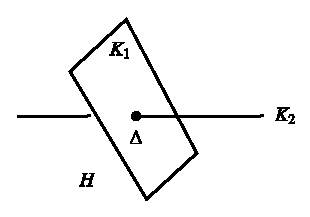
\includegraphics{figure/fig-a.eps}
\end{figure}

It follows that $\Spec R$ where $R$ is the complete local ring defined
by $\Def(C)$ is again reducible and has only two irreducible
components. 


\begin{remark}\label{part1-rem13.4}
It\pageoriginale has been shown by Pinkham that $R$ is reduced, that
the irreducible component corresponding to scrolls is of dimension $2$
and the one corresponding to Veronese is of dimension $1$, that they
are smooth, and that they intersect at the unique point corresponding
to $\overline{C}$ having normal crossings at this point.
\end{remark}

\begin{remark}\label{part1-rem13.5}
The above argument can be extended to show that $\Spec R$ for $n\geq
4$ is {\em irreducible}. Pinkham shows $\Spec R$ has an embedded
component at the point corresponding to $\overline{C}$ and outside
this it corresponds to scrolls.
\end{remark}

\begin{remark}\label{part1-rem13.6}
The reason that for $n=4$ we have got two components is that in this
case the cone over the rational quartic is a determinantal variety in
two ways, namely, it can be defined by $(2\times 2)$ minors of
$$
\begin{bmatrix}
x_{0} & \ldots & x_{3}\\
x_{1} & \ldots & x_{4}
\end{bmatrix}
\quad\text{or of}\quad 
\begin{bmatrix}
x_{0} & x_{2} & x_{4}\\
x_{2} & x_{1} & x_{3}\\
x_{4} & x_{3} & x_{2}
\end{bmatrix}
$$
\end{remark}

\begin{remark}\label{part1-rem13.7}
{\em Case $n\leq 4$.} Exercise: Discuss. 
\end{remark}
